\documentclass[../../main/main.tex]{subfiles}
\graphicspath{{./figures/}}

\dominitoc
\faketableofcontents

% \renewcommand{\mtcSfont}{\small\bfseries}
% \renewcommand{\mtcSSfont}{\footnotesize}
\mtcsettitle{minitoc}{}
\mtcsetrules{*}{off}

\makeatletter
\renewcommand{\@chapapp}{\'Electrocin\'etique -- chapitre}
\renewcommand{\chaplett}{E}
\renewcommand{\thefigure}{\chaplett\thechapter.\arabic{figure}}
\makeatother

% \toggletrue{student}
% \toggletrue{corrige}
% \renewcommand{\mycol}{black}
% \renewcommand{\mycol}{gray}

\hfuzz=5.003pt

\begin{document}
\setcounter{chapter}{6}

\settype{book}
\settype{prof}
\settype{stud}

\chapter{Oscillateurs en régime sinusoïdal forcé}

\vspace*{\fill}

\begin{tcn}(appl)<ctc>"somm"'t'{Sommaire}
	\let\item\olditem
	\vspace{-15pt}
	\minitoc
	\vspace{-25pt}
\end{tcn}

\begin{tcn}[sidebyside](appl)<ctc>"how"'t'{Capacités exigibles}
	\begin{itemize}[label=\rcheck]
		\item Oscillateur électrique ou mécanique soumis à une excitation
		      sinusoïdale.
		\item Utiliser la représentation complexe pour étudier le régime forcé.
	\end{itemize}
	\tcblower
	\begin{itemize}[label=\rcheck]
		\item Relier l'acuité d'une résonance au facteur de qualité.
		\item Déterminer la pulsation propre et le facteur de qualité à partir de
		      graphes expérimentaux d’amplitude et de phase.
	\end{itemize}
\end{tcn}

\vspace{-20pt}

% \vspace*{\fill}
% \newpage
% \vspace*{\fill}

%\vspace{-15pt}
\begin{tcn}[%
		sidebyside, fontupper=\small, fontlower=\small
	](appl)<ctb>"chek"'t'{L'essentiel}
	\begin{tcn}[nsp](defi)<ctc>'t'{Définitions}
		\vspace{-25pt}
		\tcblistof[\subsubsection*]{defi}{\hspace*{4.8pt}}
	\end{tcn}
	% \begin{tcn}[nsp](rapp)<ctc>'t'{Rappels}
	% 	\vspace{-25pt}
	% 	\tcblistof[\subsubsection*]{rapp}{\hspace*{4.8pt}}
	% \end{tcn}
	\begin{tcn}[nsp](prop)<ctc>'t'{Propriétés}
		\vspace{-25pt}
		\tcblistof[\subsubsection*]{prop}{\hspace*{4.8pt}}
		% \tcblistof[\subsubsection*]{loi}{\hspace*{4.8pt}}
		% \tcblistof[\subsubsection*]{theo}{\hspace*{4.8pt}}
	\end{tcn}
	% \begin{tcn}[nsp](loi)<ctc>'t'{Lois}
	% 	\tcblistof[\subsubsection*]{loi}{\hspace*{4.8pt}}
	% \end{tcn}
	% \begin{tcn}[nsp](coro)<ctc>'t'{Corollaires}
	%   \tcblistof[\subsubsection*]{coro}{\hspace*{4.8pt}}
	% \end{tcn}
	% \begin{tcn}[nsp](demo)<ctc>'t'{Démonstrations}
	% 	\tcblistof[\subsubsection*]{demo}{\hspace*{4.8pt}}
	% 	\tcblistof[\subsubsection*]{prev}{\hspace*{4.8pt}}
	% \end{tcn}
	% \begin{tcn}[nsp](inte)<ctc>'t'{Interprétations}
	% 	\tcblistof[\subsubsection*]{inte}{\hspace*{4.8pt}}
	% \end{tcn}
	% \begin{tcn}[nsp](impl)<ctc>'t'{Implications}
	% 	\vspace{-25pt}
	% 	\tcblistof[\subsubsection*]{impl}{\hspace*{4.8pt}}
	% \end{tcn}
	% \begin{tcn}[nsp](tool)<ctc>'t'{Outils}
	% 	\tcblistof[\subsubsection*]{tool}{\hspace*{4.8pt}}
	% \end{tcn}
	% \begin{tcn}[nsp](nota)<ctc>'t'{Notations}
	% 	\tcblistof[\subsubsection*]{nota}{\hspace*{4.8pt}}
	% \end{tcn}
	% \begin{tcn}[nsp](appl)<ctc>'t'{Applications}
	% 	\tcblistof[\subsubsection*]{appl}{\hspace*{4.8pt}}
	% \end{tcn}
	% \begin{tcn}[nsp](rema)<ctc>'t'{Remarques}
	%   \tcblistof[\subsubsection*]{rema}{\hspace*{4.8pt}}
	% \end{tcn}
	% \begin{tcn}[nsp](exem)<ctc>'t'{Exemples}
	%   \tcblistof[\subsubsection*]{exem}{\hspace*{4.8pt}}
	% \end{tcn}
	% \begin{tcn}[nsp](ror)<ctc>"hart"'t'{Points importants}
	%   \tcblistof[\subsubsection*]{ror}{\hspace*{4.8pt}}
	% \end{tcn}
	% \begin{tcn}[nsp](impo)<ctc>'t'{Erreurs communes}
	%   \tcblistof[\subsubsection*]{impo}{\hspace*{4.8pt}}
	% \end{tcn}
	\tcblower
	% \begin{tcn}[nsp](defi)<ctc>'t'{Définitions}
	%   \tcblistof[\subsubsection*]{defi}{\hspace*{4.8pt}}
	% \end{tcn}
	% \begin{tcn}[nsp](rapp)<ctc>'t'{Rappels}
	%   \tcblistof[\subsubsection*]{rapp}{\hspace*{4.8pt}}
	% \end{tcn}
	% \begin{tcn}[nsp](prop)<ctc>'t'{Propriétés}
	% \tcblistof[\subsubsection*]{prop}{\hspace*{4.8pt}}
	% \tcblistof[\subsubsection*]{loi}{\hspace*{4.8pt}}
	% \tcblistof[\subsubsection*]{theo}{\hspace*{4.8pt}}
	% \end{tcn}
	% \begin{tcn}[nsp](coro)<ctc>'t'{Corollaires}
	%   \tcblistof[\subsubsection*]{coro}{\hspace*{4.8pt}}
	% \end{tcn}
	\begin{tcn}[nsp](demo)<ctc>'t'{Démonstrations}
		\vspace{-25pt}
		\tcblistof[\subsubsection*]{demo}{\hspace*{4.8pt}}
		% \tcblistof[\subsubsection*]{prev}{\hspace*{4.8pt}}
	\end{tcn}
	% \begin{tcn}[nsp](inte)<ctc>'t'{Interprétations}
	% 	\tcblistof[\subsubsection*]{inte}{\hspace*{4.8pt}}
	% \end{tcn}
	% \begin{tcn}[nsp](impl)<ctc>'t'{Implications}
	% 	\tcblistof[\subsubsection*]{impl}{\hspace*{4.8pt}}
	% \end{tcn}
	% \begin{tcn}[nsp](tool)<ctc>'t'{Outils}
	% 	\vspace{-25pt}
	% 	\tcblistof[\subsubsection*]{tool}{\hspace*{4.8pt}}
	% \end{tcn}
	% \begin{tcn}[nsp](nota)<ctc>'t'{Notations}
	% 	\tcblistof[\subsubsection*]{nota}{\hspace*{4.8pt}}
	% \end{tcn}
	% \begin{tcn}[nsp](odgr)<ctc>'t'{Ordres de grandeur}
	% 	\tcblistof[\subsubsection*]{odgr}{\hspace*{4.8pt}}
	% \end{tcn}
	% \begin{tcn}[nsp](appl)<ctc>'t'{Applications}
	% 	\vspace{-25pt}
	% 	\tcblistof[\subsubsection*]{appl}{\hspace*{4.8pt}}
	% \end{tcn}
	% \begin{tcn}[nsp](rema)<ctc>'t'{Remarques}
	%   \tcblistof[\subsubsection*]{rema}{\hspace*{4.8pt}}
	% \end{tcn}
	% \begin{tcn}[nsp](exem)<ctc>'t'{Exemples}
	% 	\tcblistof[\subsubsection*]{exem}{\hspace*{4.8pt}}
	% \end{tcn}
	\begin{tcn}[nsp](ror)<ctc>"hart"'t'{Points importants}
		\vspace{-25pt}
		\tcblistof[\subsubsection*]{ror}{\hspace*{4.8pt}}
	\end{tcn}
	% \begin{tcn}[nsp](impo)<ctc>'t'{Erreurs communes}
	% 	\vspace{-25pt}
	% 	\tcblistof[\subsubsection*]{impo}{\hspace*{4.8pt}}
	% \end{tcn}
\end{tcn}

\vspace*{\fill}

\newpage

Parmi les systèmes soumis à une excitation sinusoïdale, les oscillateurs ont une
place d'importance par l'émergence d'une propriété remarquable~: celle de la
\textbf{résonance}. Regardons deux exemples.

\section{Exemple d'oscillateur~: circuit RLC série en RSF}
\subsection{Présentation}

\begin{tcb}(defi){RLC série en RSF}
	On s'intéresse au circuit suivant, composé d'une résistance, d'une bobine et
	d'un condensateur $C$, alimentés par un GBF. On suppose une phase nulle pour
	le signal entrant~:
	\[
		e(t) = E_0 \cos(\wt)
		\qMath{ainsi}
		u_C(t) = U_C \cos(\wt+\f_u)
		\qet
		i(t) = I \cos(\wt+\f_i)
	\]
	\tcblower
	\begin{center}
		\sswitch{%
			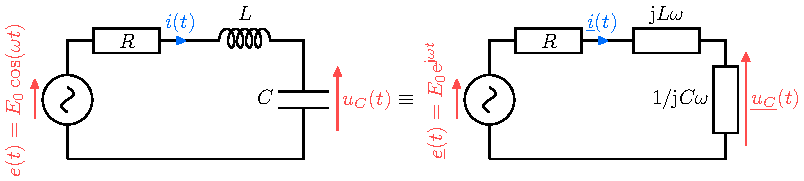
\includegraphics[width=\linewidth, draft=true]{rlc_sinu}
		}{%
			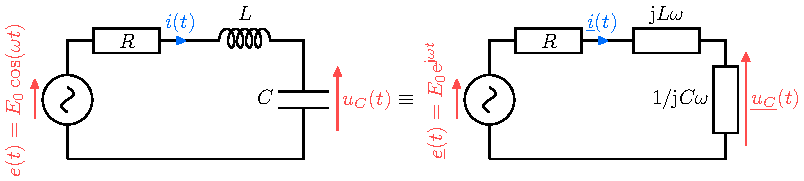
\includegraphics[width=\linewidth]{rlc_sinu}
		}%
		\captionof{figure}{RLC série en RSF.}
	\end{center}
\end{tcb}

\subsection{Étude de l'intensité}
\subsubsection{Amplitude complexe}
\begin{tcb}(prop){Amplitude complexe $\Iu$}
	L'amplitude complexe de l'intensité dans un RLC série s'écrit~:
	\begin{gather*}
		\psw{
			\boxed{
				\Iu(x) = \frac{E_0/R}{1 + \jj Q \left( x - \dfrac{1}{x} \right)}}
		}
		\qav
		\psw{\boxed{x = \frac{\w}{\w_0}}}
		\qet
		\psw{\boxed{\w_0 = \frac{1}{\sqrt{LC}}}}
		\qet
		\psw{\boxed{Q = \frac{1}{R}\sqrt{\frac{L}{C}}}}
	\end{gather*}
	\vspace{-15pt}
\end{tcb}

% TODO: Démo modifiée pour être plus explicite sur l'identification, vérifier
%  que ça passe.

\begin{tcb*}[breakable](demo){Amplitude complexe $\Iu$}
	Pour étudier le comportement de l'intensité, on va comme d'habitude se
	ramener à une seule maille avec une impédance équivalente
	% \[\Zu\ind{eq} = \Zu_R + \Zu_L + \Zu_C\]
	\smallbreak
	\vspace{-15pt}
	\begin{isd}[righthand ratio=.30]
		\psw{%
			\begin{DispWithArrows*}[fleqn, mathindent=5pt]
				E_0 = \Zu\ind{eq}\Iu & =
				\left( R + \jlw + \frac{1}{\jcw} \right)\Iu
				\Arrow{Isole\\$1/\jj = -\jj$}
				\\\Lra
				\Iu                    & =
				\frac{E_0}{R + \jj \left( L\w - \dfrac{1}{C\w} \right)}
				\Arrow{Forme canonique}
				\\\Lra
				\Iu                    & =
				\frac{E_0/R
				}{
					1 + \jj
					\bigg(
					\underbracket[1pt]{\dfrac{L}{R}}_{\mathclap{= \frac{Q}{\w_0}}}\w -
					\underbracket[1pt]{\dfrac{1}{RC}}_{\mathclap{=Q\w_0}} \dfrac{1}{\w}
					\bigg)
				}
			\end{DispWithArrows*}
		}%
		\vspace{-15pt}
		\tcblower
		\begin{center}
			\sswitch{
				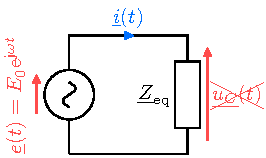
\includegraphics[width=\linewidth, draft=true]{rlc_zeq}
			}{
				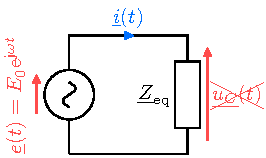
\includegraphics[width=\linewidth]{rlc_zeq}
			}
			\vspace{-15pt}
			\captionof{figure}{}
		\end{center}
	\end{isd}
	\vspace{-15pt}
	\psw{%
		\begin{align*}
			% \beforetext{On identifie alors~:}
			\frac{L}{R} = \frac{Q}{\w_0}
			\quad & \text{et} \quad
			\frac{1}{RC} = Q\w_0
			\\\Lra
			\frac{\frac{1}{RC}}{\frac{L}{R}} =
			\frac{Q\w_0}{\frac{Q}{\w_0}}
			\Lra
			\w_0{}^2 = \frac{1}{LC}
			\quad & \text{et} \quad
			\frac{L}{R} \times \frac{1}{RC} = Q^2
			\Lra
			Q^2 = \frac{1}{R^2} \frac{L}{C}
			\\\Lra
			\boxed{\w_0 = \frac{1}{\sqrt{LC}}}
			\quad & \text{et} \quad
			\boxed{Q = \frac{1}{R}\sqrt{\frac{L}{C}}}
		\end{align*}
	}%
	D'où le résultat.
	\hqed
\end{tcb*}

\subsubsection{Solution réelle}

\begin{tcb}(prop){$i(t)$ RLC série en RSF}
	\leftcenters{%
		L'intensité réelle s'écrit donc
	}{%
		$i(t) = I(x) \cdot \cos(\wt + \f_i(x))$
	}%
	\smallbreak
	\begin{isd}[interior hidden, sidebyside align=top](prop)
		\tcbsubtitle{\fatbox{\textbf{Amplitude réelle}}}
		\psw{%
			\[
				\boxed{
					I(x)
					= \abs{\Iu}
					= \frac{E_0/R}{\sqrt{1 + Q^2\left( x - \dfrac{1}{x} \right)^2}}
				}
			\]
		}%
		\vspace{-15pt}
		\tcblower
		\tcbsubtitle{\fatbox{\textbf{Phase}}}
		\vspace{-15pt}
		\begin{gather*}
			\psw{%
				\boxed{\f_i = - \arctan(Q \left( x - \frac{1}{x} \right))}
			}%
			\\\text{avec}
			\quad
			\psw{%
			\f_i \in \left] -\frac{\pi}{2}\,; \frac{\pi}{2} \right[
			}%
		\end{gather*}
		\vspace{-15pt}
	\end{isd}
\end{tcb}

\begin{tcb*}[%
		sidebyside, sidebyside align=top, lefthand ratio=.25%
	](demo){$i(t)$ RLC série en RSF}
	\tcbsubtitle{\fatbox{\textbf{Amplitude réelle}}}
	C'est évident.
	\tcblower
	\tcbsubtitle{\fatbox{\textbf{Phase}}}
	\vspace{-15pt}
	\psw{
		\begin{gather*}
			\f_i
			= \underbracket[1pt]{\cancel{\arg*{E_0/R}}}_{=0}
			- \arg*{1 + \jj Q \left( x - \frac{1}{x} \right)}
			\\\Ra
			\tan(\f_i) =
			- \tan\/(%
			\arg{%
			\underbracket[1pt]{1}_{\mathclap{\Re > 0}} +
			\jj Q\left( x - \frac{1}{x} \right)
			}
			)
			\\\Lra
			\boxed{\f_i = -\arctan(Q \pa{x - \frac{1}{x}})}
			\qavec
			\boxed{\f_i \in \left] - \frac{\pi}{2}\,; \frac{\pi}{2} \right[}
		\end{gather*}
	}
\end{tcb*}

\subsubsection{Notion de résonance et bande passante}
Par l'étude de l'amplitude, on retrouve bien que $\Iu$ ne dépend pas des
conditions initiales, mais bien de l'amplitude d'entrée et surtout
\textbf{dépend de la pulsation}. Notamment, on trouve que
\begin{gather*}
	\psw{
		\boxed{I \xrightarrow[x\to+\infty]{} 0}
	}
	\qet
	\psw{
		\boxed{I \xrightarrow[x\to0]{} 0}
	}
\end{gather*}

Ainsi, il y a une valeur particulière de pulsation telle que l'amplitude est
maximale~: c'est ce qu'on appelle la \textbf{résonance}.

\begin{tcb}(defi){Résonance}
	Un oscillateur forcé présente une résonance si l'\textbf{amplitude de ses
		oscillations est maximale} pour une \textbf{fréquence de forçage finie
		et non nulle}.
	\smallbreak
	La fréquence correspondante est appelée \textbf{fréquence de
		résonance} $f_r$ (ou $\w_r$ ou $x_r$).
	\smallbreak
	Soit, pour une amplitude réelle $X(\w)$,
	\psw{%
		\begin{gather*}
			\exists
			\text{résonance}
			\quad \Lra \quad
			\boxed{\exists \w_r \neq (0,+\infty)~:~ X(\w_r) = X_{\max}}
		\end{gather*}
	}%
	\vspace{-15pt}
\end{tcb}

La représentation de l'amplitude en fonction de la pulsation est donc piquée
autour de son maximum $X_{\max}$ à la pulsation de résonance $\w_r$. Ce pic peut
être plus ou moins fin, ce que l'on caractérise par la \textbf{bande passante}.
\begin{tcb*}[sidebyside, righthand ratio=.4](defi){Bande passante}
	C'est le domaine de pulsations du forçage défini par~:
	\psw{
		\[
			\text{bande passante}
			\triangleq
			\left\{%
			\w ~|~ X(\w) \geq X\ind{max, eff} = \frac{X\ind{max}}{\sqrt{2}}\right
			\}
			% \boxed{X(\w) > X\ind{max, eff} = \frac{X\ind{max}}{2}}
		\]
	}
	\begin{itemize}
		\item $\w_1$ et $\w_2$ les \textbf{pulsations de coupure}, telles que
		      \psw{%
			      \[
				      X(\w_{1,2}) = \frac{X\ind{max}}{\sqrt{2}}
			      \]
		      }%
		      \vspace{-15pt}
		\item la \textbf{bande passante}
		      \psw{%
			      $\quad \D\w = \abs{\w_2 - \w_1}$~;
		      }%
		\item l'\textbf{acuité de la résonance}
		      \psw{%
			      $\quad \w_r/\D\w$.
		      }%
	\end{itemize}
	\tcblower
	\begin{center}
		\sswitch{%
			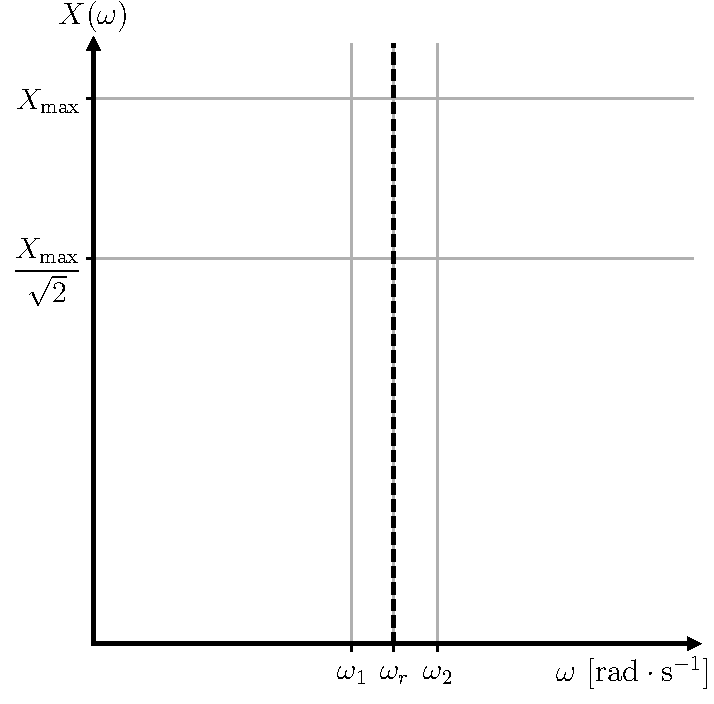
\includegraphics[width=.8\linewidth]{bande_pass_stud}
		}{%
			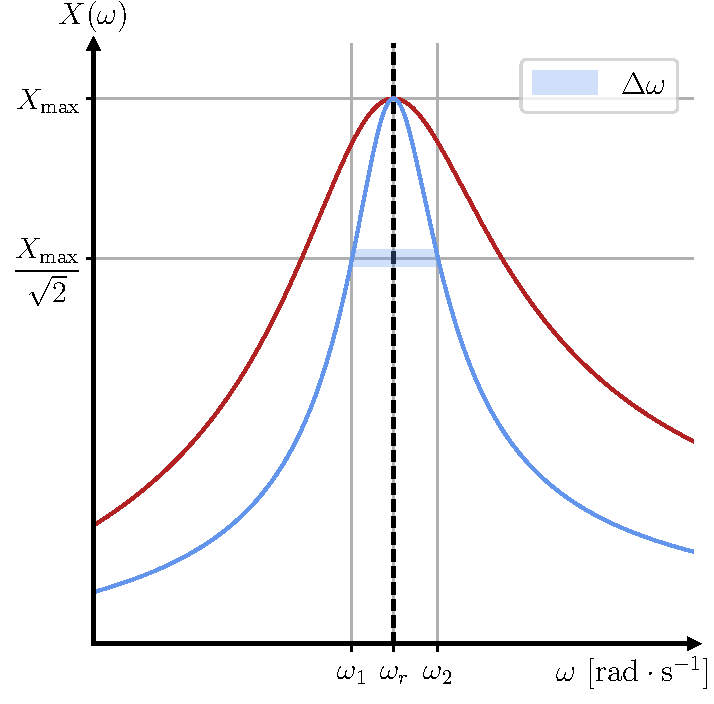
\includegraphics[width=.8\linewidth]{bande_pass_prof}
		}%
		\vspace{-15pt}
		\captionof{figure}{Bande passante.}
	\end{center}
\end{tcb*}

\subsubsection{Comportements à la résonance}

\begin{tcb*}(prop){Résonance en intensité RLC série}
	La pulsation de résonance en intensité est~:
	\[
		\psw{%
			\boxed{\w_r = \w_0}
		}%
		\quad \Lra \quad
		\psw{%
			\boxed{x_r = 1}
		}
	\]
	\begin{isd}[interior hidden](prop)
		\tcbsubtitle{\fatbox{\textbf{Amplitude de résonance}}}
		\psw{%
			\[
				\boxed{I(x_r) = I\ind{max} = \frac{E_0}{R}}
			\]
		}%
		\vspace{-15pt}
		\tcblower
		\tcbsubtitle{\fatbox{\textbf{Phase à la résonance}}}
		\psw{%
			\[
				\boxed{\f_i(x_r) = 0}
			\]
		}%
		\vspace{-15pt}
	\end{isd}
\end{tcb*}

\begin{tcb*}[breakable](demo){Résonance en intensité RLC série}
	\tcbsubtitle{\fatbox{\textbf{Amplitude de résonance}}}
	On trouve la résonance en trouvant le \textbf{maximum de l'amplitude réelle}.
	\smallbreak
	Ici, \xul{comme le numérateur est constant}, il suffit d'avoir
	\textbf{le dénominateur minimal}~:
	\begin{gather*}
		\psw{%
			I(x_r) = I_{\max}
			\Lra
			1 + \underbracket[1pt]{Q^2\left( x_r - \frac{1}{x_r} \right)^2}_{\geq 0}
			\quad \text{minimal}
		}%
		\\\Lra
		\psw{%
			Q^2\left( x_r - \frac{1}{x_r} \right)^2 = 0
			\Lra
			x_r = \frac{1}{x_r}
		}%
		\\\Lra
		\psw{%
			\boxed{x_r = 1}
			\qou
			\boxed{\w_r = \w_0}
		}%
	\end{gather*}
	\vspace{-15pt}
	\tcblower
	\tcbsubtitle{\fatbox{\textbf{Phase à la résonance}}}
	On reprend l'étude de l'argument faite précédemment~:
	\psw{%
	\[
		\tan(\f_i(x_r)) = - Q \pa{x_r - \frac{1}{x_r}} = 0
		\Lra
		\boxed{\f_i(x_r) = 0}
		\qcr
		\f_i \in \left] -\frac{\pi}{2}\,; \frac{\pi}{2} \right[
	\]
	}%
	\vspace{-15pt}
\end{tcb*}

\subsubsection{Bande passante et facteur de qualité}
Nous avons déterminé l'amplitude et la phase du signal, ainsi que la
pulsation de résonance. Pour finir de caractériser la résonance, il ne reste
qu'à déterminer la bande passante.

\begin{tcb*}(prop){Bande passante et facteur de qualité}
	Plus le facteur de qualité est grand, plus la résonance est sélective. On
	relie la bande passante à la pulsation propre et au facteur de qualité
	\textit{via} la relation~:
	\[
		\psw{%
			\boxed{%
				\Delta{\w} = \frac{\w_0}{Q}
				\Lra
				Q = \frac{\w_0}{\Delta{\w}}
			}
		}%
	\]
	On retrouve l'\textbf{acuité de la résonance}.
\end{tcb*}

\begin{tcb*}[breakable](demo){Bande passante et facteur de qualité}
	On cherche donc les pulsations de coupure réduites telles que $I(x_k) =
		I\ind{max, eff} = \frac{I_{\max}}{\sqrt{2}}$~:
	\begin{DispWithArrows*}[%
			format=RrL, fleqn, xoffset=2.5cm
		]%
		&
		\psw{I(x_k)}
		&=
		\psw{\frac{I\ind{max}}{\sqrt{2}}}
		\Arrow{On remplace}
		\\\Lra
		&
		\qquad \qquad \qquad \qquad
		\psw{\frac{E_0/R}{\sqrt{1 + Q^2 \pa{x_k - \frac{1}{x_k}} ^2}}}
		&=
		\psw{\frac{E_0/R}{\sqrt{2}}}
		\Arrow{On isole}
		\\\Lra
		& \Aboxed{
			\psw{Q^2 \pa{x_k - \frac{1}{x_r}}^2}
			&=
			\psw{1}
		}
		\CArrow{$\sqrt{\cdot}$}
		\\\Lra
		&
		\psw{Q \pa{x_k - \frac{1}{x_k}}}
		&=
		\psw{\pm 1}
		\Arrow{$\times x_k$}
		\\\Lra
		&
		\psw{Qx_k{}^2 - Q}
		&=
		\psw{\pm x_k}
		\Arrow{$-\pm = \mp$}
		\\\Lra
		&
		\psw{Q x_i{}^{2} \mp x_k - Q}
		&=
		\psw{0}
		\intertext{On a alors \textbf{deux trinômes}, soit \textbf{quatre racines
				possibles}.}
		% \Arrow{Discriminant}
		\Ra &
		\psw{\Delta}
		&=
		\psw{1 + 4Q{}^{2}}
		\Arrow{Solutions}
		\\\Ra
		&
		\psw{x_{i,\pm,\pm}}
		&=
		\psw{\frac{\pm 1 \pm \sqrt{1+4Q{}^{2}}}{2Q}}
	\end{DispWithArrows*}
	\vspace{-15pt}
	On ne garde que les racines positives, sachant que
	$\boxed{\sqrt{1+4Q{}^{2}} > 1}$~:
	\begin{DispWithArrows*}[]
		\psw{%
		x_1 = x_{k,-,+} = \frac{1}{2Q} \pa{-1 + \sqrt{1+4Q{}^{2}}}
		}%
		\quad &\text{et} \quad
		\psw{%
		x_2 = x_{k,+,+} = \frac{1}{2Q} \pa{1 + \sqrt{1+4Q{}^{2}}}
		}%
	\end{DispWithArrows*}
	puis on obtient la bande passante en calculant la différence $\abs{x_2 -
			x_1}$~:
	\psw{%
		\[
			x_2 - x_1 =
			\frac{1+\cancel{\sqrt{1+4Q^2}} - \pa{-1 + \cancel{\sqrt{1+4Q^2}}}}{2Q}
			\Lra
			\boxed{\Delta{x} = \frac{1}{Q} \Lra \Delta{\w} = \frac{\w_0}{Q}}
			\qed
		\]
	}%
\end{tcb*}

\begin{tcb}(ror){À retenir pour $\Iu$}
	\begin{itemize}
		\item \psw{%
			      Il n'y a \textbf{aucune condition} pour avoir résonance~: celle-ci
			      existe peu importe le facteur de qualité~;
		      }%
		\item \psw{%
			      La \textbf{pulsation de résonance} est \textbf{égale à la pulsation
				      propre}~;
		      }%
		\item \psw{%
			      L'\textbf{amplitude maximale} ne \textbf{dépend pas de $Q$}~;
		      }%
		\item \psw{%
			      La \textbf{phase à la résonance} est \textbf{nulle}.
		      }%
	\end{itemize}
	\begin{isd}
		\begin{center}
			\sswitch{%
				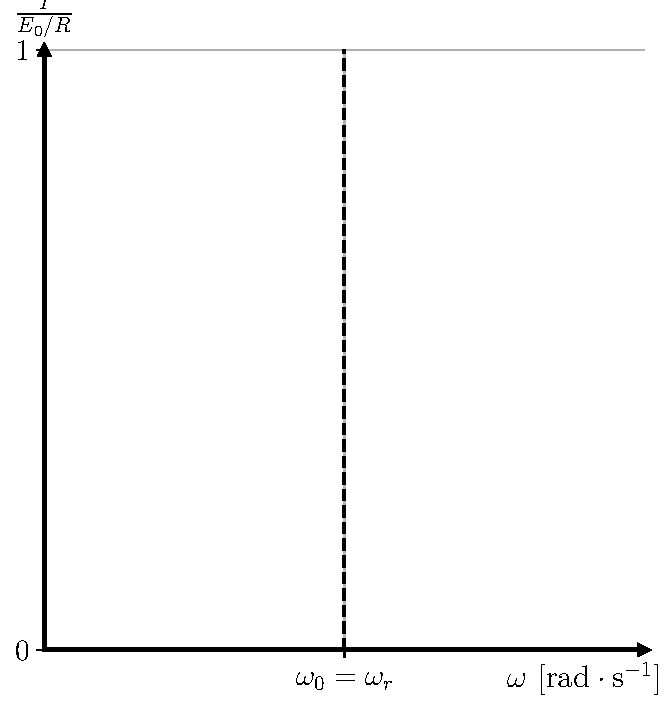
\includegraphics[height=7.5cm]{rlc_I_ampl_stud}
			}{%
				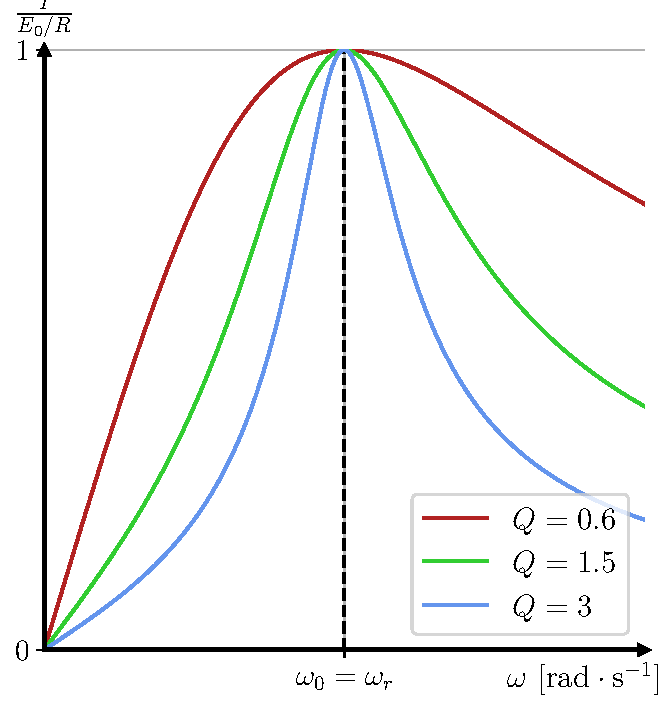
\includegraphics[height=7.5cm]{rlc_I_ampl_prof}
			}%
			\captionof{figure}{$\abs{\Iu}$ selon $Q$.}
		\end{center}
		\tcblower
		\begin{center}
			\sswitch{%
				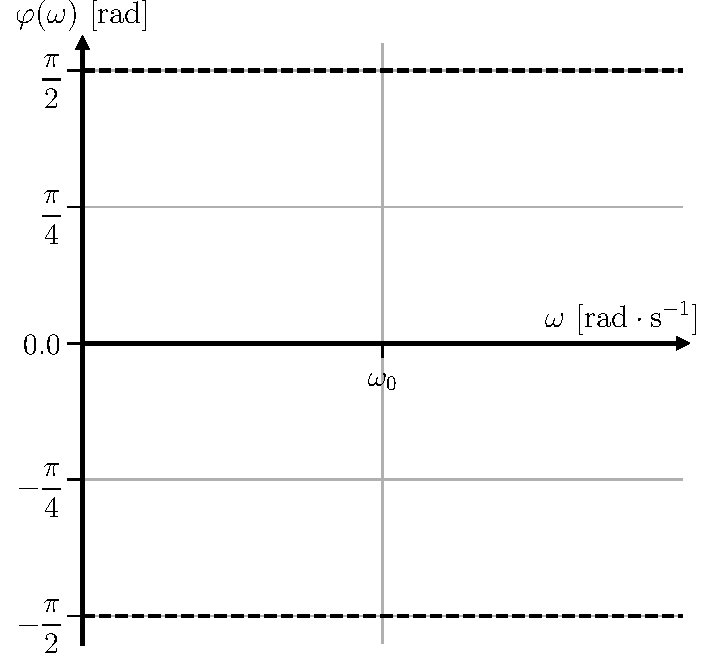
\includegraphics[height=7.5cm]{rlc_I_arg_stud}
			}{%
				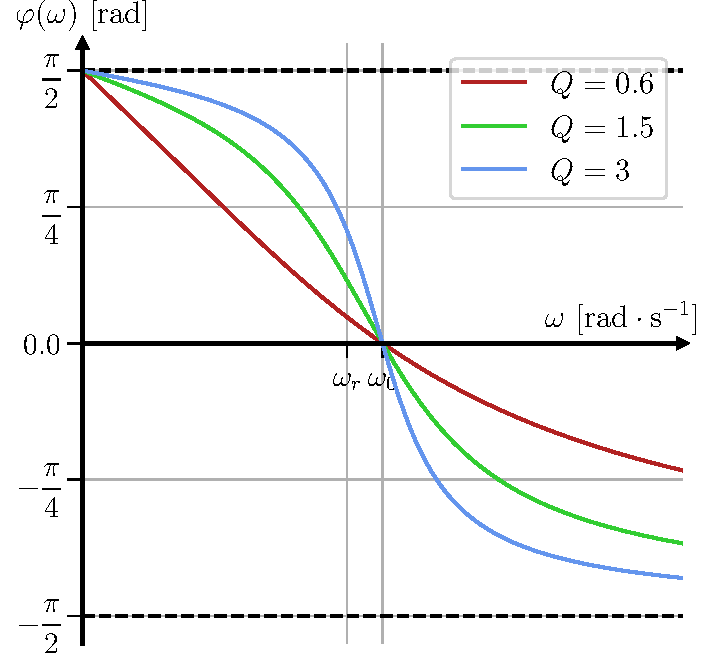
\includegraphics[height=7.5cm]{rlc_I_arg_prof}
			}%
			\vspace{-15pt}
			\captionof{figure}{$\arg*{\Iu}$ selon $Q$.}
		\end{center}
	\end{isd}
	% \begin{center}
	% 	\sswitch{
	% 		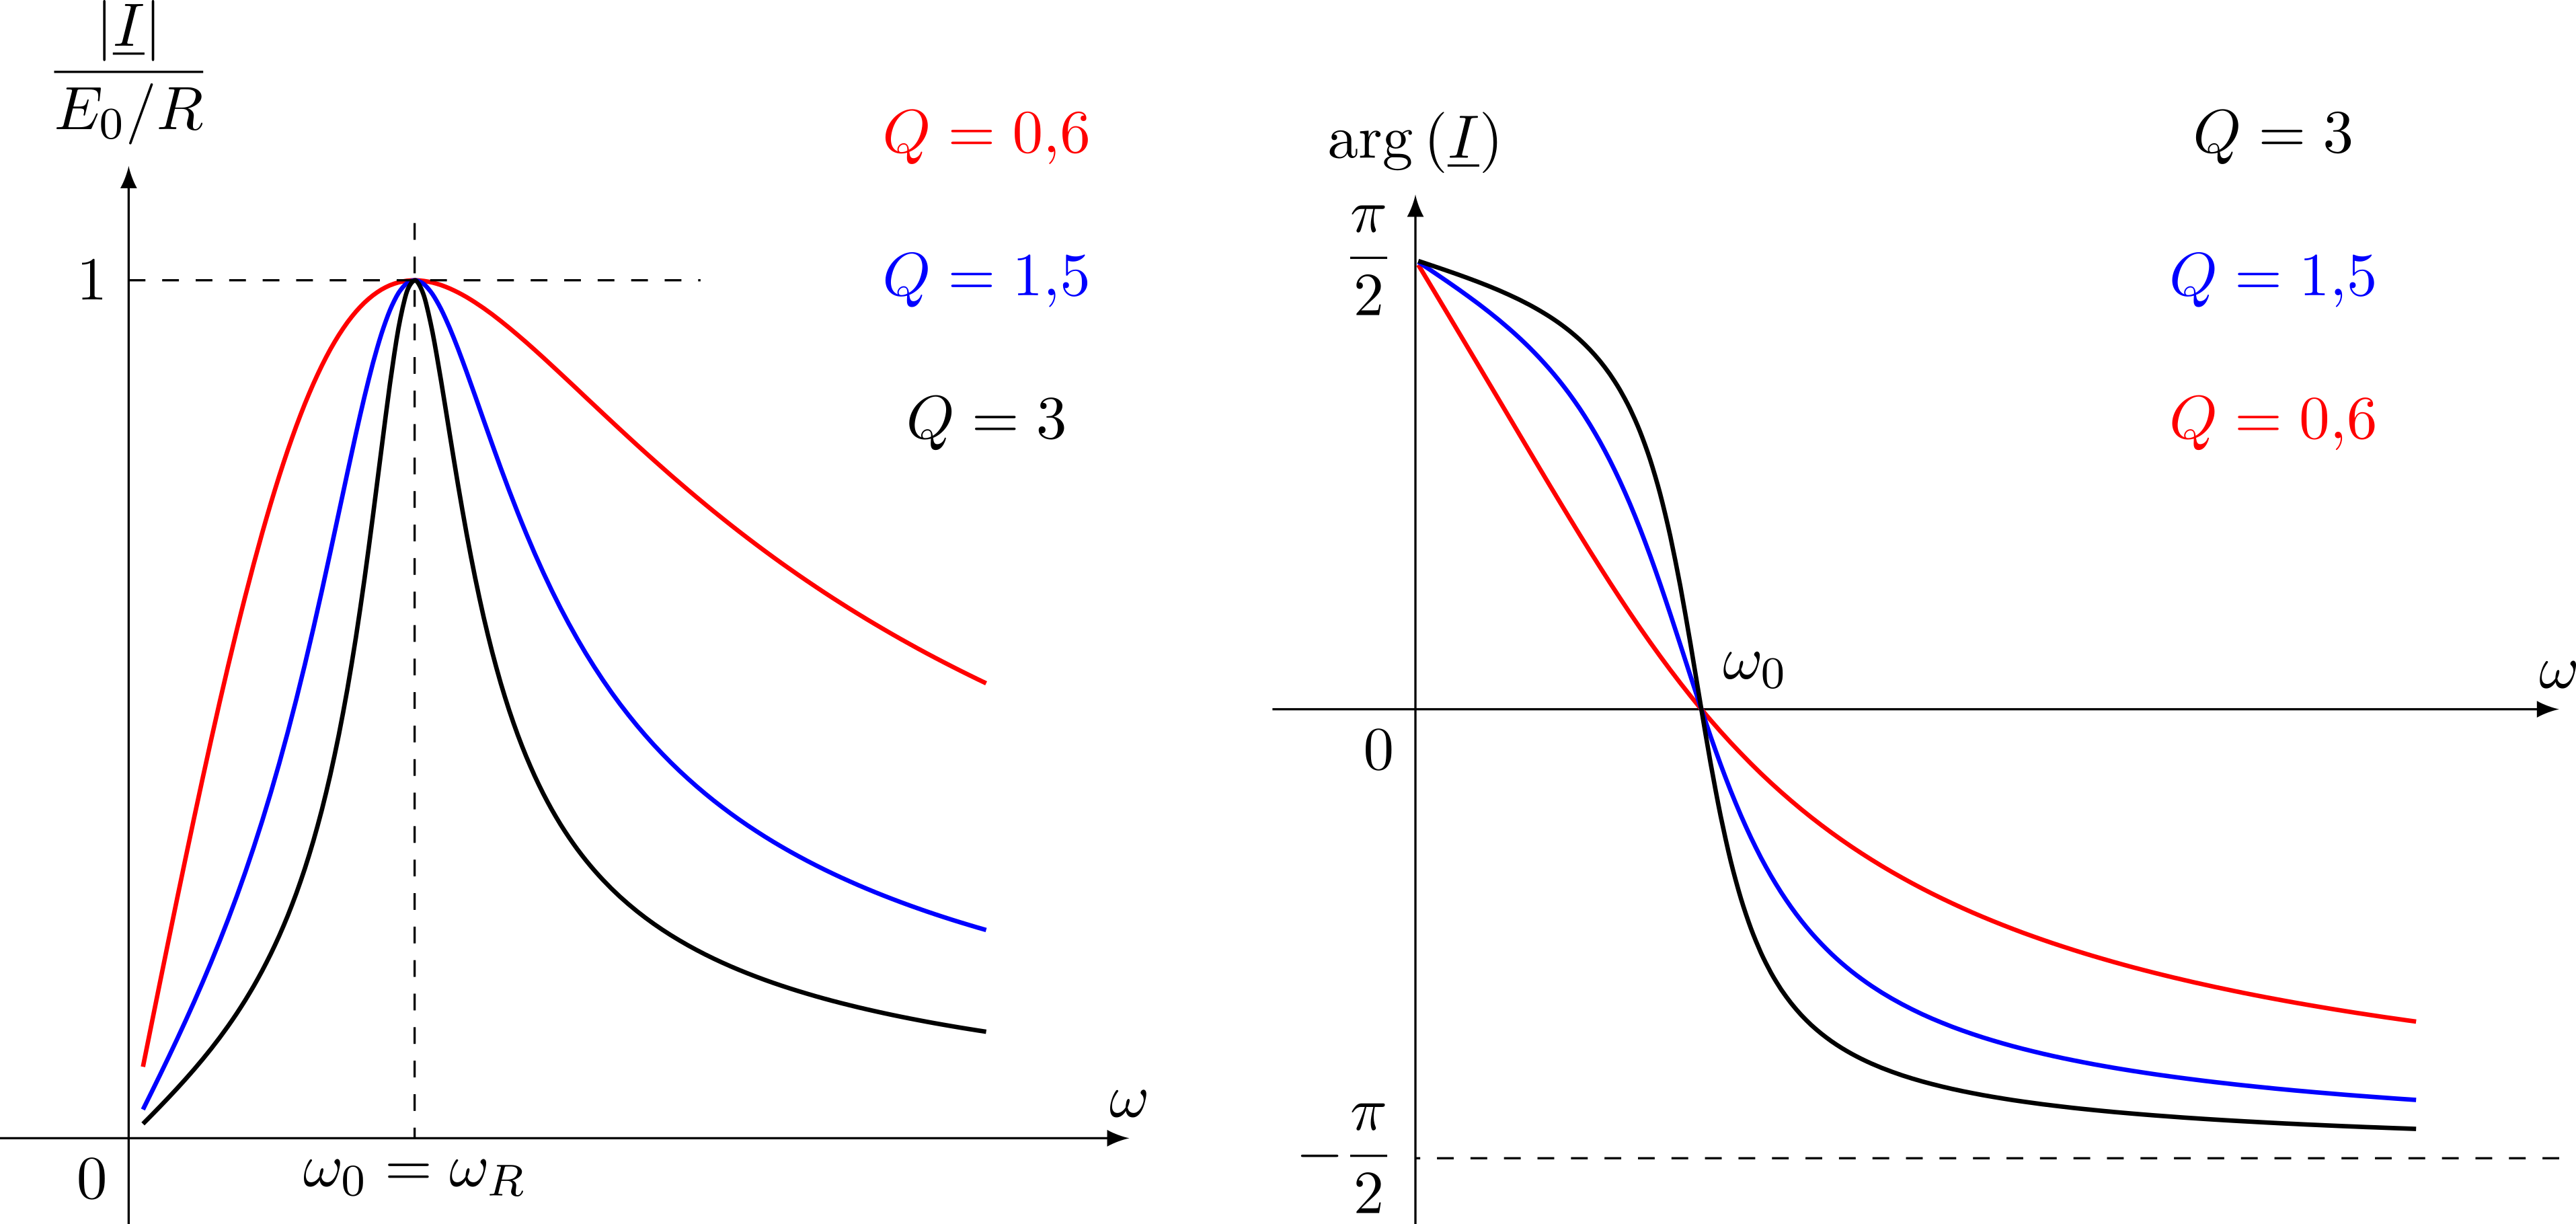
\includegraphics[width=.8\linewidth, draft=true]{rlc_i-ampphase}
	% 	}{
	% 		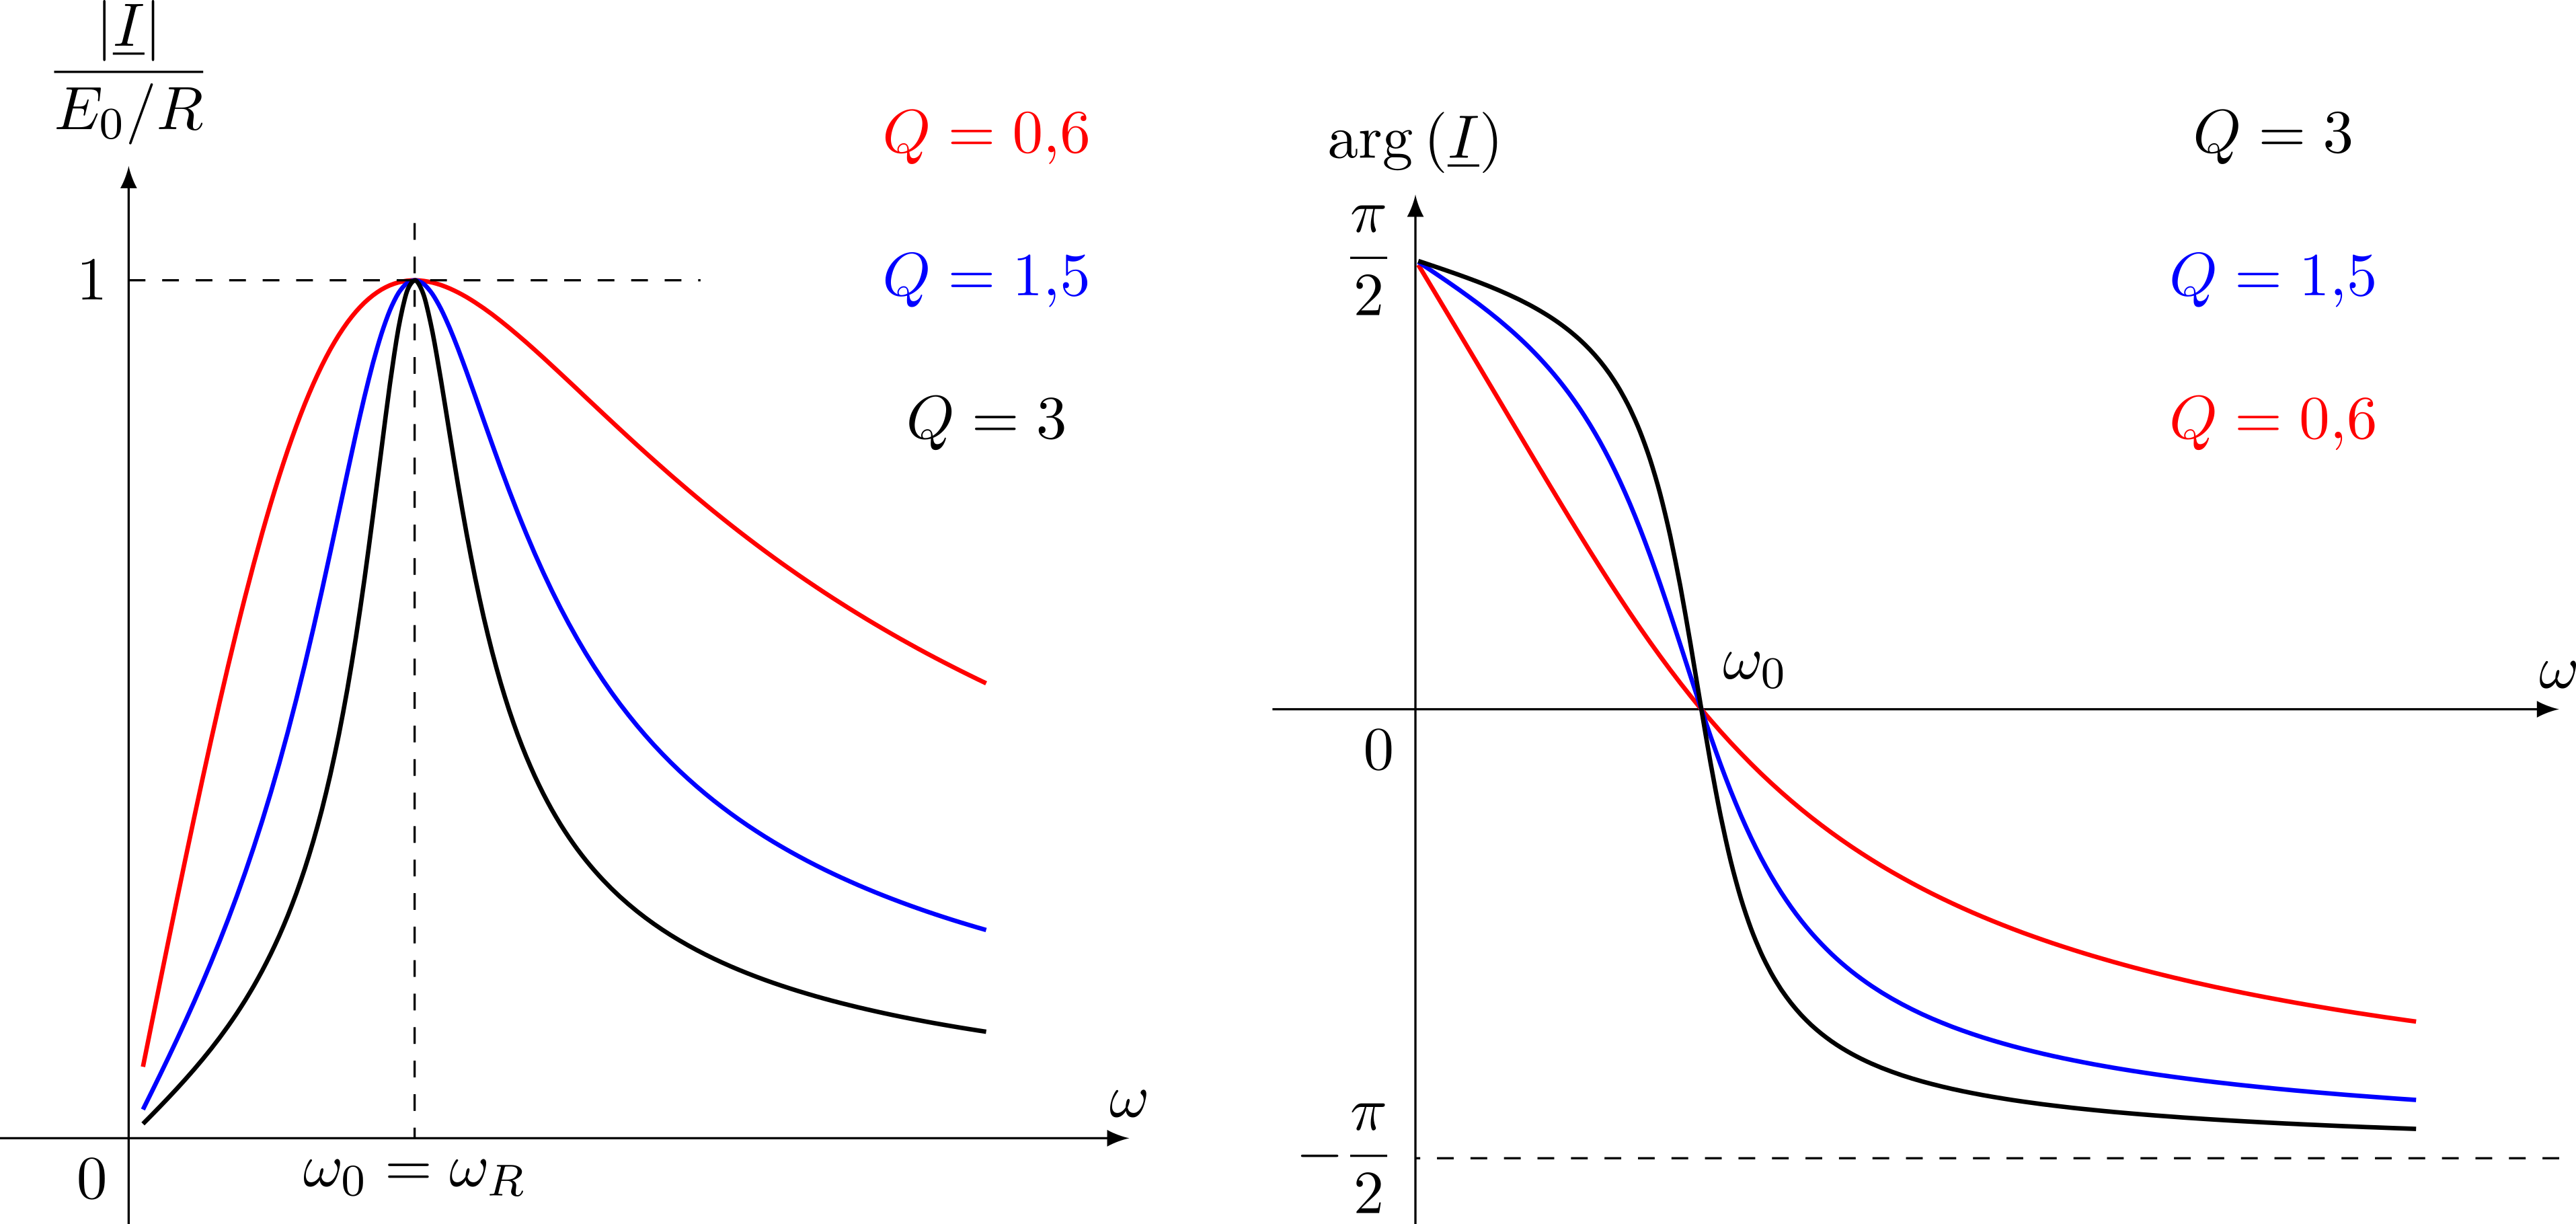
\includegraphics[width=.8\linewidth]{rlc_i-ampphase}
	% 	}
	% 	\captionof{figure}{Amplitude et phase en fonction de $Q$ pour $\Iu$ en RLC
	% 		série.}
	% \end{center}
\end{tcb}

\subsection{Étude de la tension $u_C$}
On repart du circuit en complexes, avec $\xul{u_C}(t) = \Uu\exr^{\jwt}$ et
$\eu(t) = E\exr^{\jwt}$, et on applique le pont diviseur de tension.

\subsubsection{Amplitude complexe $\Uu_C$}
\begin{tcb}(prop){Amplitude complexe $\Uu_C$}
	L'amplitude complexe de la tension du condensateur d'un RLC série s'écrit~:
	\[
		\psw{%
			\boxed{\Uu_C(x) = \frac{E_0}{1-x^2 + \jj \dfrac{x}{Q}}}
		}%
		\qav
		\psw{\boxed{x = \frac{\w}{\w_0}}}
		\qet
		\psw{\boxed{\w_0 = \frac{1}{\sqrt{LC}}}}
		\qet
		\psw{\boxed{Q = \frac{1}{R}\sqrt{\frac{L}{C}}}}
	\]
\end{tcb}

\begin{tcb*}[sidebyside](demo){Amplitude complexe $\Uu_C$}
	\begin{center}
		\sswitch{
			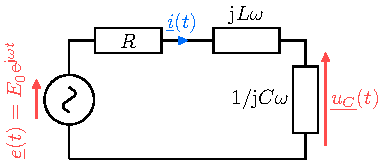
\includegraphics[width=\linewidth, draft=true]{rlc_u-circ}
		}{
			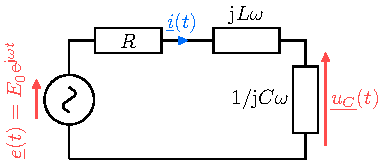
\includegraphics[width=\linewidth]{rlc_u-circ}
		}
		\vspace{-15pt}
		\captionof{figure}{RLC série~: étude de $\uu_C$.}
	\end{center}
	\tcblower
	\psw{
		\begin{DispWithArrows*}[fleqn, mathindent=5pt]
			\Uu &= \frac{1/\jcw}{R + \jlw + 1/\jcw}E_0
			\CArrow{$\times \jcw$}
			\\\Lra
			\Uu &= \frac{E_0}{1 - (LC\w)^2 + \jj RC\w}
			\Arrow{$\w_0$ et $Q$}
			\\\Lra
			\Aboxed{
				\Uu &=
				\frac{E_0}{1 -
					\left( \dfrac{\w}{\w_0} \right)^2 +
					\jj\dfrac{\w}{Q\w_0}}
			}
			\qed
		\end{DispWithArrows*}
	}
\end{tcb*}

\subsubsection{Solution réelle}
\begin{tcb}(prop){$u_C(t)$ RLC série en RSF}
	\leftcenters{%
		La tension réelle s'écrit donc
	}{%
		$u_C(t) = U_C(x) \cdot \cos(\wt + \f_u(x))$
	}%
	\smallbreak
	\begin{isd}[interior hidden, sidebyside align=top](prop)
		\tcbsubtitle{\fatbox{\textbf{Amplitude réelle}}}
		\psw{%
			\[
				\boxed{
					U(x)
					= \abs{\Uu}
					= \frac{E_0}{
						\sqrt{ \pa{1 - x^2} ^2 + \pa{\dfrac{x}{Q}}^2}}
				}
			\]
		}%
		\vspace{-15pt}
		\tcblower
		\tcbsubtitle{\fatbox{\textbf{Phase}}}
		\begin{gather*}
			\psw{%
				\boxed{\tan(\f_u(x)) = - \frac{x}{Q \pa{1 - x^2}}}
			}%
			\\\text{avec}
			\quad
			\psw{%
			\f_u \in \left] -\pi\,; 0 \right[
			}%
		\end{gather*}
		\vspace{-15pt}
	\end{isd}
\end{tcb}

\begin{tcb*}[%
		sidebyside, sidebyside align=top, lefthand ratio=.25%
	](demo){$u_C(t)$ RLC série en RSF}
	\tcbsubtitle{\fatbox{\textbf{Amplitude réelle}}}
	C'est évident.
	\tcblower
	\tcbsubtitle{\fatbox{\textbf{Phase}}}
	\vspace{-15pt}
	\psw{%
		\begin{gather*}
			\f_u
			= \underbracket[1pt]{\cancel{\arg*{E_0}}}_{=0}
			- \arg*{1 - x^2 + \jj \frac{x}{Q}}
			\\\Ra
			\tan(\f_u) =
			- \tan\/(%
			\overbracket[1pt]{%
			\arg{%
			\underbracket[1pt]{1 - x^2}_{\mathclap{\Re \lessgtr 0}} +
			\jj \underbracket[1pt]{\frac{x}{Q}}_{\mathclap{\Im > 0}}
			}
			}^{\in ]0 \,; \pi[}
				)
				\\\Lra
				\boxed{\tan(\f_u(x)) = - \frac{x}{Q \pa{1 - x^2}}}
				\\\text{avec}
				\quad
				\f_u \in \left] -\pi\,; 0 \right[
			\qed
		\end{gather*}
	}%
	\vspace{-15pt}
\end{tcb*}

\subsubsection{Comportements à la résonance}

\begin{tcb*}[breakable](prop){Résonance en tension du RLC série}
	La résonance en tension n'\textbf{existe pas toujours}~:
	\begin{itemize}[leftmargin=60pt]
		\item{}[$\mathbf{Q \leq 1/\sqrt{2}}$] :
		      \textbf{pas de résonance}, l'amplitude est maximale pour
		      \psw{%
			      \[\boxed{x = 0 \qet U(0) = E_0}\]
		      }%
		      \vspace{-15pt}
		\item{}[$\mathbf{Q > 1/\sqrt{2}}$] :
		      La résonance existe, l'amplitude est maximale pour
		      \psw{%
			      \[
				      \boxed{x_r = \frac{1}{Q} \sqrt{Q^{2} - \frac{1}{2}} < 1}
				      \qet
				      \boxed{U(x_r) = \frac{QE}{\sqrt{1 - \frac{1}{4Q^{2}}}}}
			      \]
		      }%
		      \vspace{-15pt}
		\item{}[$\mathbf{Q > 5}$] :
		      \leavevmode\vspace*{-15pt}\relax
		      \psw{%
			      \[
				      \boxed{x_r \approx 1}
				      \Lra
				      \boxed{\w_r \approx \w_0}
				      \qet
				      \boxed{U(x_r) \approx QE}
			      \]
		      }%
		      \vspace{-15pt}
	\end{itemize}
\end{tcb*}

\begin{tcb*}[breakable](demo){Résonance en tension du RLC série}
	\tcbsubtitle{\fatbox{\textbf{Condition de résonance}}}
	On trouve le maximum de l'amplitude quand le dénominateur est
	\textbf{non nul} et minimal, c'est-à-dire
	\vspace{-15pt}
	\psw{
		\begin{gather*}
			U(x_r) = U_{\max}
			\Lra
			\left( 1 - x^2 \right)^2 + \pa{\dfrac{x}{Q}}^2
			\quad
			\text{minimal}
		\end{gather*}
	}
	Soit $X = x^2$, et $f(X) = \left(1 - X\right)^2 + \dfrac{X}{Q^2}$, la
	fonction que l'on cherche à minimiser~: on cherche $X_r$ tel que \textbf{sa
		dérivée s'annule}, c'est-à-dire
	\psw{%
		\begin{DispWithArrows*}
			f'(X_r) &= 0
			\Arrow{On dérive}
			\\\Lra
			-2 \left( 1-X_r \right) + \frac{1}{Q^2} &= 0
			\Arrow{On isole}
			\\\Lra
			X_r-1 = - \frac{1}{2Q^2}
			& \Lra
			X_r = 1 - \frac{1}{2Q^2}
			\Arrow{$X_r = x^{2}$}
			\\\Lra
			x_r = \sqrt{1 - \frac{1}{2Q^2}}
			& \Lra
			\boxed{
				x_r = \frac{1}{Q} \sqrt{Q^{2} - \frac{1}{2}}
			}
		\end{DispWithArrows*}
	}%
	ce qui n'est défini \textbf{que si} $Q > \dfrac{1}{\sqrt{2}}$. Si $Q <
		\frac{1}{\sqrt{2}}$, alors le maximum se trouve en $\w = 0$, ce qui n'est
	\textbf{pas une résonance} puisqu'il n'y a alors \textbf{pas d'excitation}.
	\tcblower
	\tcbsubtitle{\fatbox{\textbf{Amplitude de résonance}}}
	\smallbreak
	\begin{isd}[righthand ratio=.4]
		On calcule alors $f(X_r)$ en injectant la solution~:
		\psw{%
			\begin{DispWithArrows*}[fleqn, mathindent=5pt, groups]
				f(X_r) &=
				\left( \cancel{1} -
				\left( \cancel{1} - \frac{1}{2Q^{2}} \right)
				\right)^{2} +
				\frac{1}{Q^{2}} \left( 1 - \frac{1}{2Q^{2}} \right)
				% \Arrow{On simplifie et développe}
				\\\Lra
				f(X_r) &=
				\left( \frac{1}{2Q^{2}} \right)^{2} + \frac{1}{Q^{2}} - \frac{1}{2Q^{4}}
				\Arrow{Même dénom.}
				\\\Lra
				f(X_r) &=
				\frac{1}{4Q^{2}} - \frac{2}{4Q^{4}} + \frac{1}{Q^{2}}
				\Arrow{On calcule}
				\\\Lra
				f(X_r) &=
				\frac{1}{Q^{2}} - \frac{1}{4Q^{4}}
				\Arrow{On factorise}
				\\\Lra
				\Aboxed{%
					f(X_r) &=
					\frac{1}{Q^{2}}\left( 1 - \frac{1}{4Q^{2}} \right)
				}
			\end{DispWithArrows*}
		}
		\vspace{-15pt}
		\tcblower
		Dans $U(x)$~:
		\psw{%
			\begin{DispWithArrows*}[fleqn, mathindent=5pt]
				\Ra
				U(x_r) &= \frac{E_0}{\sqrt{f(X_r)}}
				\CArrow{$\sqrt{(\cdot)}$}
				\\\Lra
				U(x_r) &= \frac{E_0}{
					\frac{1}{Q}\sqrt{1 - \frac{1}{4Q^{2}}}
				}
				\Arrow{Simplifie}
				\\\Lra
				\Aboxed{U(x_r) &= \frac{QE_0}{\sqrt{1 - \frac{1}{4Q^{2}}}}}
			\end{DispWithArrows*}
		}
	\end{isd}
	\vspace{-15pt}
\end{tcb*}

\begin{tcb}(ror){À retenir pour $\Uu_C$}
	\begin{itemize}
		\item \psw{%
			      Il y \textbf{a une condition} pour avoir résonance,
			      $Q>\frac{1}{\sqrt{2}}$, elle s'obtient par étude de fonction~;
		      }%
		\item \psw{%
			      La \textbf{pulsation de résonance} est \textbf{différente de la
				      pulsation propre} mais s'en rapproche avec $Q \nearrow$~;
		      }%
		\item \psw{%
			      L'\textbf{amplitude maximale dépend de $Q$}~: $Q \nearrow \Ra
				      U\ind{max} \nearrow$~;
		      }%
		\item \psw{%
			      La \textbf{phase à la résonance} est \textbf{quelconque}~;
		      }%
		\item \psw{%
			      La \textbf{phase à la pulsation propre} est $\f_u(\w_0) =
				      -\frac{\pi}{2}$~;
		      }%
	\end{itemize}
	\begin{isd}
		\vspace{-15pt}
		\begin{center}
			\sswitch{%
				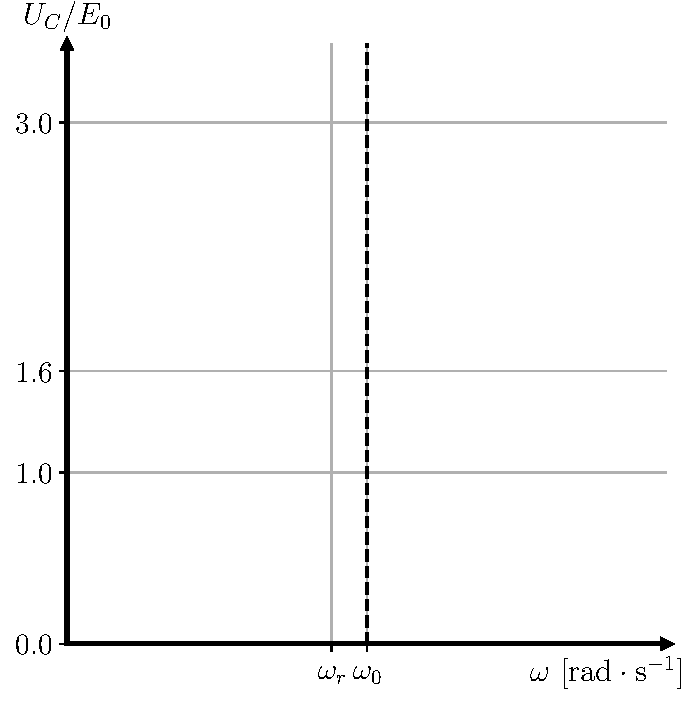
\includegraphics[height=7cm]{rlc_Uc_ampl_stud}
			}{%
				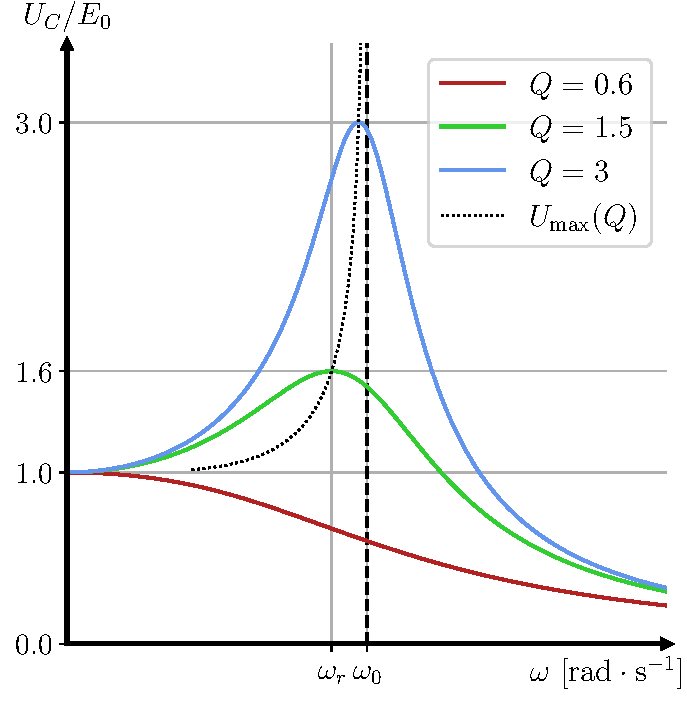
\includegraphics[height=7cm]{rlc_Uc_ampl_prof}
			}%
			\captionof{figure}{$\abs{\Uu}$ selon $Q$.}
		\end{center}
		\tcblower
		\vspace{-15pt}
		\begin{center}
			\sswitch{%
				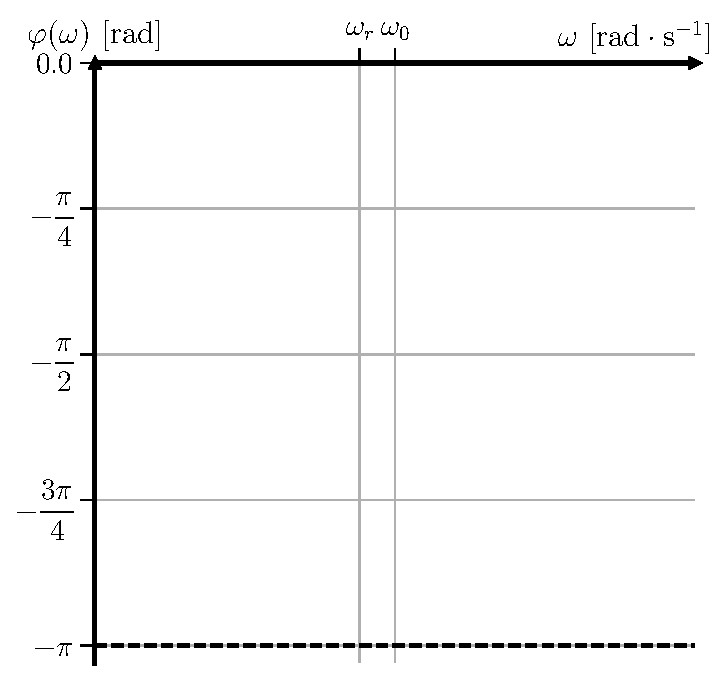
\includegraphics[height=7cm]{rlc_Uc_arg_stud}
			}{%
				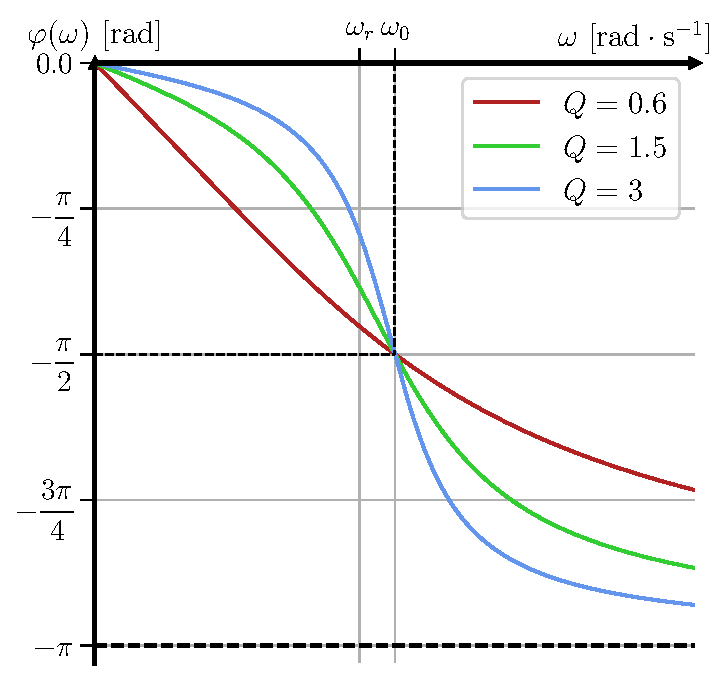
\includegraphics[height=7cm]{rlc_Uc_arg_prof}
			}%
			\captionof{figure}{$\arg*{\Uu}$ selon $Q$.}
		\end{center}
	\end{isd}
	% \begin{center}
	% 	\sswitch{
	% 		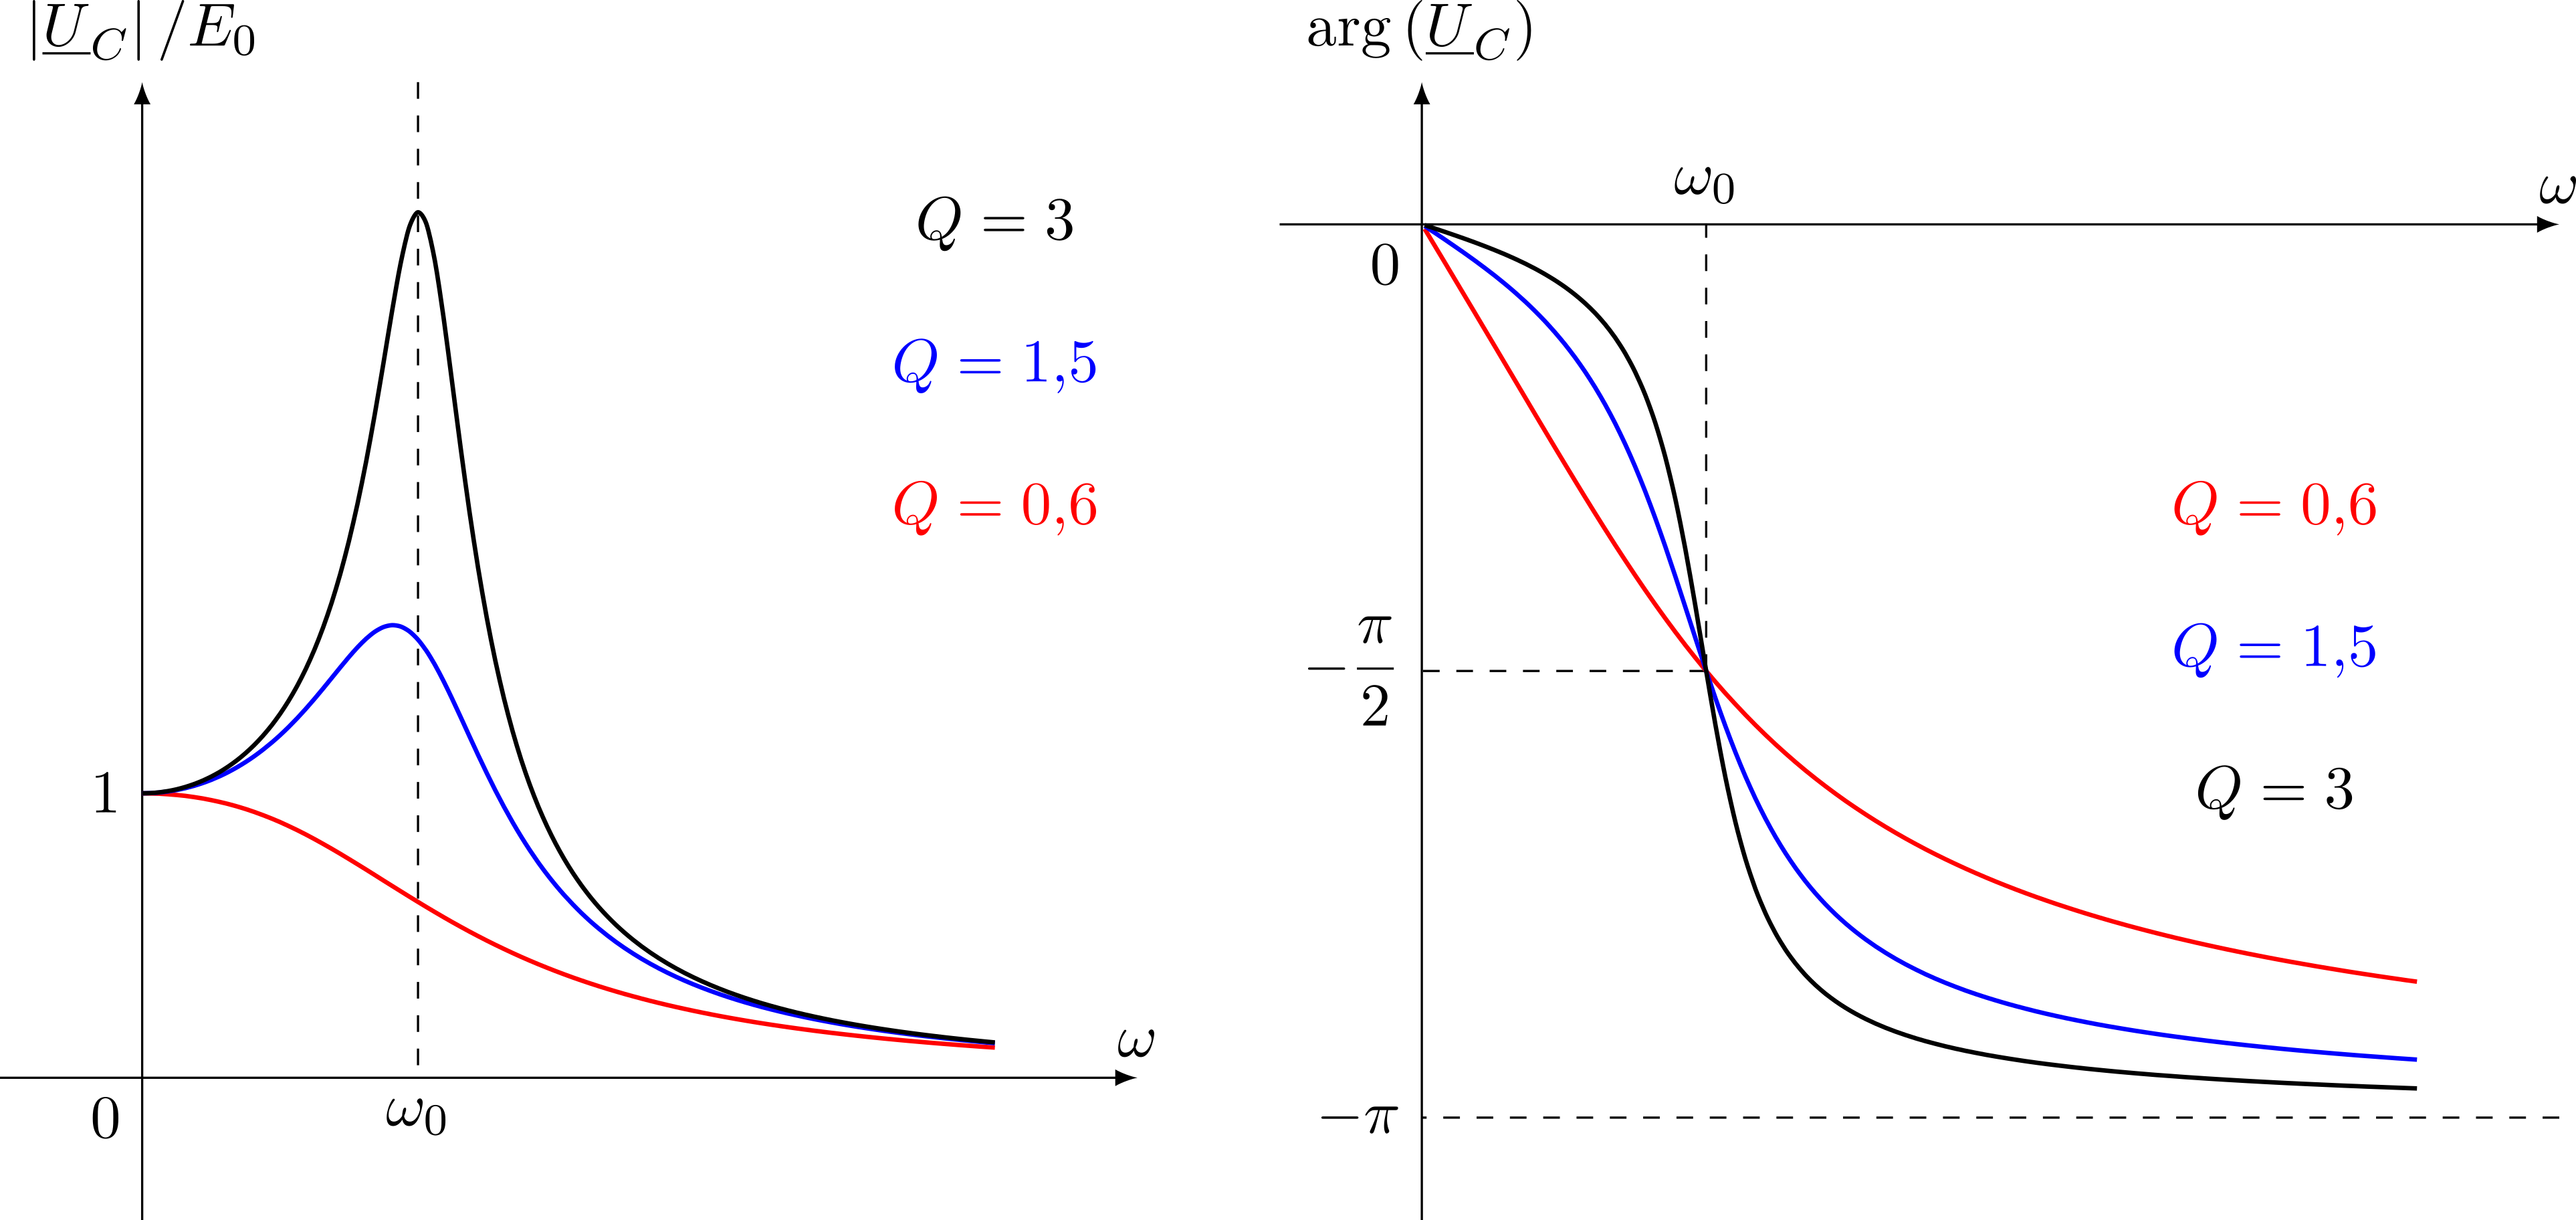
\includegraphics[width=.8\linewidth, draft=true]{rlc_u-ampphase}
	% 	}{
	% 		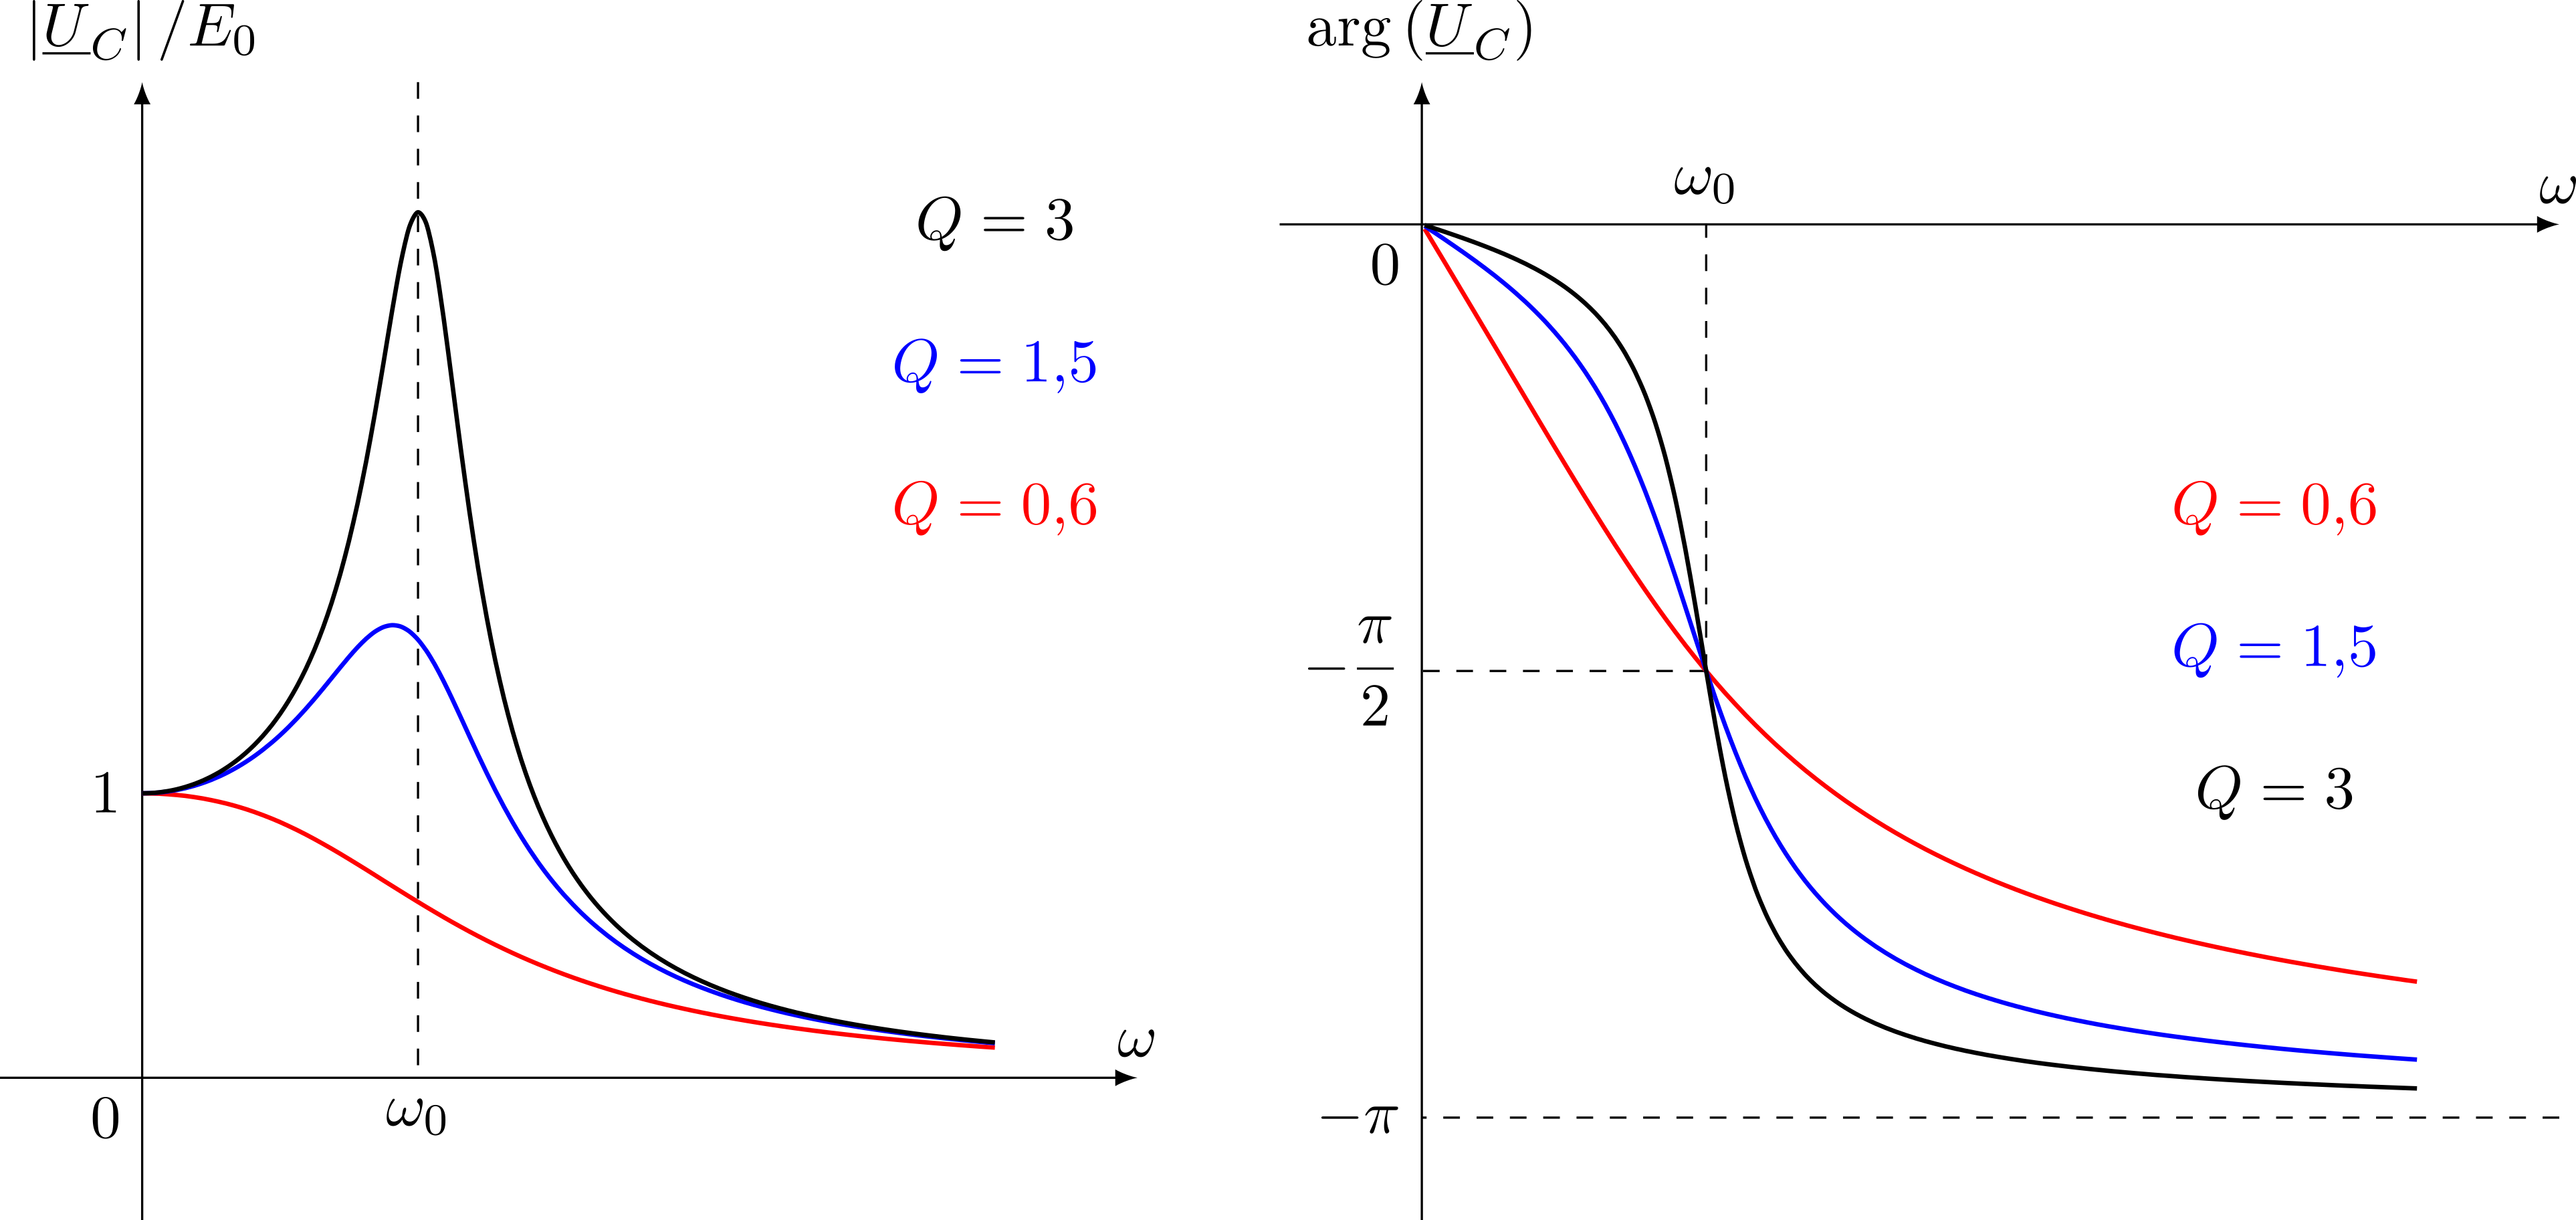
\includegraphics[width=.8\linewidth]{rlc_u-ampphase}
	% 	}
	% 	\captionof{figure}{Amplitude et phase en fonction de $Q$ pour $\Iu$ en RLC
	% 		série.}
	% \end{center}
\end{tcb}

\section{Exemple d'un oscillateur mécanique en RSF}
\subsection{Présentation}
\begin{tcb*}(defi){Ressort amorti en RSF}
	\begin{itemize}
		\item[b]{Système} : point matériel $M$ de masse $m$ relié à un ressort
		      horizontal \textbf{idéal}.
		\item[b]{Référentiel} : $\Rc_{\rm sol}$ terrestre supposé galiléen~;
		\item[b]{Repère} : $(O,\ux,\uy)$ avec $\uy$ ascendant vers le haut
		\item[b]{Repérage} :
		      \psw{%
			      \[
				      \OM(t) = \ell(t) \ux~;
				      \vf(t) = \lp(t)\ux~;
				      \af(t) = \lpp(t)\ux
			      \]
		      }%
	\end{itemize}
	\vspace{-25pt}
	\begin{isd}[righthand ratio=.45]
		\textbf{Bilan des forces}~:
		\begin{enumerate}
			\item \psw{%
				      Poids $\Pf = -mg\uy$~;
			      }%
			\item \psw{%
				      Réaction du support $\vv{R} = R\uy$~;
			      }%
			\item \psw{%
				      Force de \textsc{Hooke} $\vv*{F}{\rm ressort} = -k (\ell(t) -
					      \ell_0)\ux$~;
			      }%
			\item \psw{%
				      Force de frottement fluide $\vv*{F}{\rm frott} = -\alpha \xp(t)\ux$~;
			      }%
			\item \psw{%
				      \textbf{Force excitatrice} $\ff_e = F_0\cos(\wt)\ux$.
			      }%
		\end{enumerate}
		\tcblower
		\begin{center}
			\sswitch{
				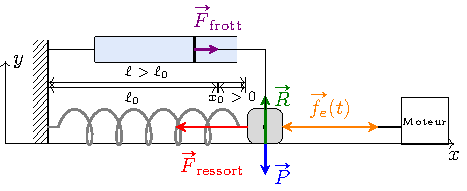
\includegraphics[width=\linewidth, draft=true]{ressort-horiz}
			}{
				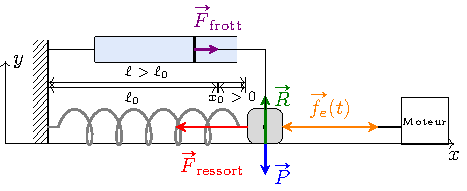
\includegraphics[width=\linewidth]{ressort-horiz}
			}
			\vspace{-15pt}
			\captionof{figure}{Schéma du ressort en RSF.}
		\end{center}
	\end{isd}
\end{tcb*}

\subsection{Étude de l'élongation}
\subsubsection{Amplitude complexe $\Xu$}

\begin{tcb}(prop){Amplitude complexe $\Xu_C$}
	L'amplitude complexe de l'élongation d'un ressort en RSF s'écrit~:
	\[
		\psw{%
			\boxed{
				\Xu(u) =
				\frac{F_0/k}{1 - u ^2 + \jj\dfrac{x}{Q}}
			}
		}%
		\qav
		\psw{\boxed{u = \frac{\w}{\w_0}}}
		\qet
		\psw{\boxed{\w_0 = \sqrt{\frac{k}{m}}}}
		\qet
		\psw{\boxed{Q = \frac{\sqrt{km}}{\alpha}}}
	\]
\end{tcb}

\begin{tcb*}[breakable](demo){Amplitude complexe $\Xu_C$}
	Avec le PFD~:
	\leavevmode\vspace*{-25pt}\relax
	\psw{%
		\begin{gather*}
			m\af = \Pf + \vv{R} + \Ff_{\rm ressort} + \Ff_{\rm frott} +\ff_e\\
			\Lra m\left(
			\begin{array}{c}
					\dv[2]{\ell}{t} \\
					0
				\end{array}
			\right)
			=
			\left(
			\begin{array}{c}
					-k (\ell(t) - \ell_0) -\alpha \dv{\ell}{t} + F_0\cos(\wt) \\
					-mg + R
				\end{array}
			\right)
		\end{gather*}
		La projection sur $\uy$ montre que $\Rf = -\Pf$. Sur l'axe $\ux$, avec le
		changement de variable $x(t) = \ell(t) - \ell_0$, on trouve
		\begin{gather*}
			m \dv[2]{x}{t} + \alpha \dv{x}{t} + kx = F_0\cos(\wt)
			\Lra
			\\
			\boxed{\xpp + \frac{\w_0}{Q}\xp + \w_0{}^2x =
				\frac{F_0}{m}\cos(\wt)}
			\qavec
			\boxed{\w_0 = \sqrt{\frac{k}{m}}}
			\qet
			\frac{\w_0}{Q} = \frac{\alpha}{m}
			\Ra
			\boxed{Q = \frac{\sqrt{km}}{\alpha}}
		\end{gather*}
	}%
	En passant en complexes,
	\leavevmode\vspace*{-25pt}\relax
	\psw{%
		\begin{DispWithArrows*}
			\pa{(\jw)^2 + \frac{\w_0}{Q}\jw + \w_0{}^2}\Xu &= \frac{F_0}{m}
			\CArrow{$\mdiv \w_0{}^2$}
			\\\Lra
			\pa{-\pa{\frac{\w}{\w_0}}^2 + \jj \frac{\w}{\w_0Q} + 1}\Xu &=
			\frac{F_0}{\w_0{}^2m}
			\Arrow{$m\w_0{}^2 = k$\\$u = \w/\w_0$}
			\\\Lra
			\Aboxed{\Xu(u) &= \frac{F_0/k}{1 - u^2 + \jj \frac{u}{Q}}}
			\qed
		\end{DispWithArrows*}
	}%
	\vspace{-15pt}
\end{tcb*}

\begin{tcb}(impo)<lftt>{Notations de pulsation réduites}
	Il peut arriver très vite de confondre $x(t)$ la position et $x = \w/\w_0$ la
	pulsation réduite, d'où la notation proposée de $u = \w/\w_0$, à ne
	pas confondre avec la tension. Soyez vigilant-es.
	\vspace{-10pt}
\end{tcb}

\vspace{-15pt}
\subsubsection{Solution réelle}
\begin{tcb}(prop){$x(t)$ ressort amorti en RSF}
	\leftcenters{%
		L'élongation réelle s'écrit donc
	}{%
		$x(t) = X(u) \cdot \cos(\wt + \f_x(u))$
	}%
	\smallbreak
	\begin{isd}[interior hidden, sidebyside align=top](prop)
		\tcbsubtitle{\fatbox{\textbf{Amplitude réelle}}}
		\vspace{-15pt}
		\psw{%
			\[
				\boxed{
					X(u)
					= \abs{\Xu}
					= \frac{F_0/k}{
						\sqrt{ \pa{1 - u^2} ^2 + \pa{\dfrac{u}{Q}}^2}}
				}
			\]
		}%
		\vspace{-15pt}
		\tcblower
		\tcbsubtitle{\fatbox{\textbf{Phase}}}
		\vspace{-15pt}
		\begin{gather*}
			\psw{%
				\boxed{\tan(\f_x(u)) = - \frac{u}{Q \pa{1 - u^2}}}
			}%
			\\\text{avec}
			\quad
			\psw{%
			\f_x \in \left] -\pi\,; 0 \right[
			}%
		\end{gather*}
		\vspace{-15pt}
	\end{isd}
\end{tcb}

\subsubsection{Comportements à la résonance}

\begin{tcb*}[breakable](prop){Résonance en élongation}
	La résonance en élongation n'\textbf{existe pas toujours}~:
	\begin{itemize}[leftmargin=60pt]
		\item{}[$\mathbf{Q \leq 1/\sqrt{2}}$] :
		      \textbf{pas de résonance}, l'amplitude est maximale pour
		      \psw{%
			      \[\boxed{u = 0 \qet X(0) = \frac{F_0}{k}}\]
		      }%
		      \vspace{-15pt}
		\item{}[$\mathbf{Q > 1/\sqrt{2}}$] :
		      La résonance existe, l'amplitude est maximale pour
		      \psw{%
			      \[
				      \boxed{u_r = \frac{1}{Q} \sqrt{Q^{2} - \frac{1}{2}} < 1}
				      \qet
				      \boxed{X(u_r) = \frac{QF_0/k}{\sqrt{1 - \frac{1}{4Q^{2}}}}}
			      \]
		      }%
		      \vspace{-15pt}
		\item{}[$\mathbf{Q > 5}$] :
		      \leavevmode\vspace*{-15pt}\relax
		      \psw{%
			      \[
				      \boxed{u_r \approx 1}
				      \Lra
				      \boxed{\w_r \approx \w_0}
				      \qet
				      \boxed{X(u_r) \approx Q\frac{F_0}{k}}
			      \]
		      }%
		      \vspace{-15pt}
	\end{itemize}
\end{tcb*}

% Vous trouverez
% ici\footnote{\href{http://www.sciences.univ-nantes.fr/sites/genevieve\_tulloue/Meca/Oscillateurs/ressort\_rsf.php?typanim=Javascript}{http://www.sciences.univ-nantes.fr/sites/genevieve\_tulloue/Meca/Oscillateurs/ressort\_rsf.php?typanim=Javascript}}
% une animation interactive d'un système similaire avec un ressort vertical.

\subsection{Résonance en vitesse}
\subsubsection{Amplitude complexe}
\begin{tcb}(prop){Amplitude complexe $\Vu$}
	L'amplitude complexe de la vitesse d'un ressort en RSF s'écrit~:
	\begin{gather*}
		\psw{
			\boxed{
				\Vu(u) = \frac{F_0/\alpha}{1 + \jj Q \left( u - \dfrac{1}{u} \right)}}
		}
		\qav
		\psw{\boxed{u = \frac{\w}{\w_0}}}
		\qet
		\psw{\boxed{\w_0 = \sqrt{\frac{k}{m}}}}
		\qet
		\psw{\boxed{Q = \frac{\sqrt{km}}{\alpha}}}
	\end{gather*}
	\vspace{-15pt}
\end{tcb}

\begin{tcb*}(demo){Amplitude complexe $\Vu$}
	\vspace{-10pt}
	\psw{%
		\begin{DispWithArrows*}
			v(t) = \dv{x}{t}
			\Lra
			\Vu &= \jw\Xu
			\\\Lra
			\Vu &= \frac{F_0}{k} \frac{\jw}{1-u^2 + \jj \frac{u}{Q}}
			\Arrow{$\times \frac{\jj }{\jj }$\\$\w = u \w_0$}
			\\\Lra
			\Vu &= - \frac{F_0}{k} \frac{u\w_0}{\jj - \jj u^2 - \frac{u}{Q}}
			\Arrow{Factorise par $u$}
			\\\Lra
			\Vu &= \frac{F_0}{k}\cdot \cancel{\frac{u}{u}} \cdot
			\frac{\w_0}{\frac{1}{Q} - \jj \pa{\frac{1}{u} - 1}}
			\CArrow{$\times \frac{Q}{Q}$}
			\\\Lra
			\Vu &= \frac{F_0}{k} \cdot \frac{Q\w_0}{1+ \jj Q \pa{u - \frac{1}{u}}}
			\Arrow{$\frac{Q\w_0}{k} = \frac{1}{\alpha}$}
			\\
			\Aboxed{\Vu(u) &= \frac{F_0/\alpha}{1 + \jj Q \left( u - \dfrac{1}{u} \right)}}
			\qed
		\end{DispWithArrows*}
	}%
\end{tcb*}

\subsubsection{Amplitude réelle}
\begin{tcb}(prop){Résonance en vitesse}
	On trouve alors
	\[
		\psw{
			\boxed{
				V_{\max} = V(\w_0) = \frac{F_0}{\alpha}
			}
		}
		\qet
		\psw{
			\boxed{
				V\xrightarrow[\w\to0^+]{} 0
			}
		}
		\qet
		\psw{
			\boxed{
				V\xrightarrow[\w\to+\infty]{} 0
			}
		}
	\]
	De ce résultat, nous observons qu'il \textbf{n'y a pas de condition pour
		avoir résonance en vitesse}, et que \textbf{la pulsation de résonance est la
		pulsation propre du système}.
\end{tcb}
%On retrouve également $Q = \w_0/\D\w$ avec $\f(\w_r) = 0$.

\vspace{-15pt}
\section{Synthèse}
\begin{tcb}[label=ror:oscrsf-synth,
		tabularx*={\renewcommand{\arraystretch}{1.8}}{M{3cm}|Y|Y}]
	(ror){Synthèse résonances}
	\textbf{Grandeur} &
	Intensité/vitesse &
	Tension/élongation
	\\\hline
	\textbf{Existence} &
	\psw{Toujours}
	&
	\psw{$Q > 1/\sqrt{2}$}
	\\\hline
	\textbf{Pulsation de résonance} &
	\psw{$\w_0$}
	&
	\psw{$\w_r \lesssim \w_0$}
	\\\hdashline
	\textbf{Largeur de résonance} &
	\psw{$\D\w = \dfrac{\w_0}{Q}$}
	&
	\psw{$\D\w \approx\dfrac{\w_0}{Q}$}
	\\\hline
	\textbf{Aspects à $\w_r$} &
	\psw{
		Maximum d'amplitude\smallbreak
		Déphasage nul, $\f = 0$
	}
	&
	\psw{
		Maximum d'amplitude
	}
	\\\hdashline
	\textbf{Aspects à $\w_0$} &
	\psw{
		Résonance
	}
	&
	\psw{
		Sortie = $Q\times$entrée\smallbreak
		Quadrature de phase, $\f = -\dfrac{\pi}{2}$
	}
	\\\hline
	\textbf{Courbes d'amplitude} &
	\sswitch{
		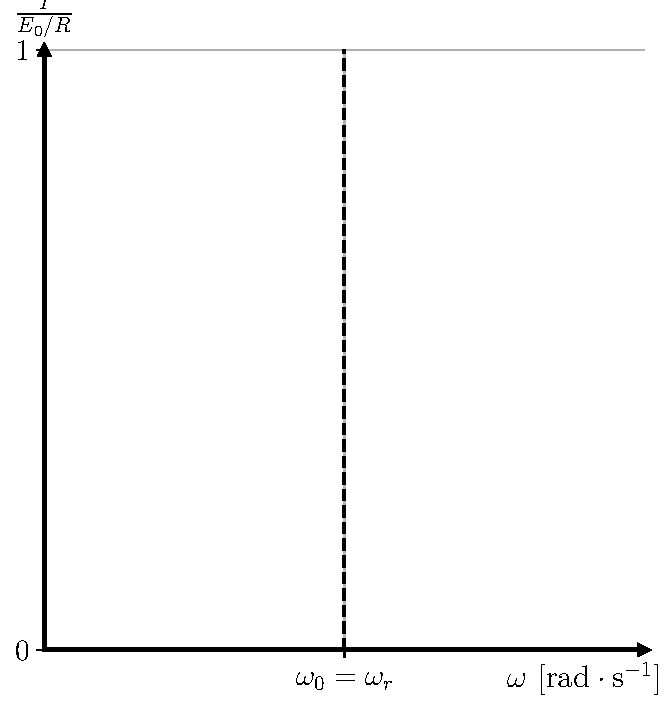
\includegraphics[width=.75\linewidth]{rlc_I_ampl_stud}
	}{
		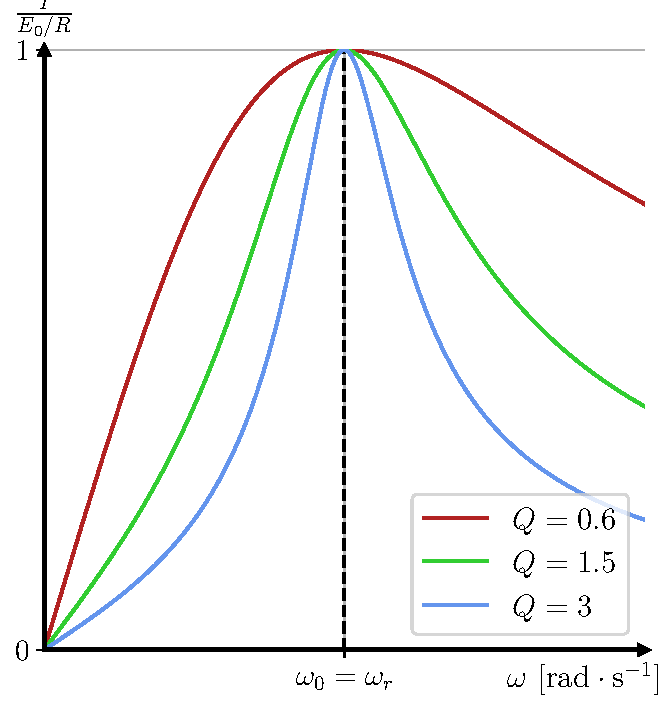
\includegraphics[width=.75\linewidth]{rlc_I_ampl_prof}
	}
	&
	\sswitch{
		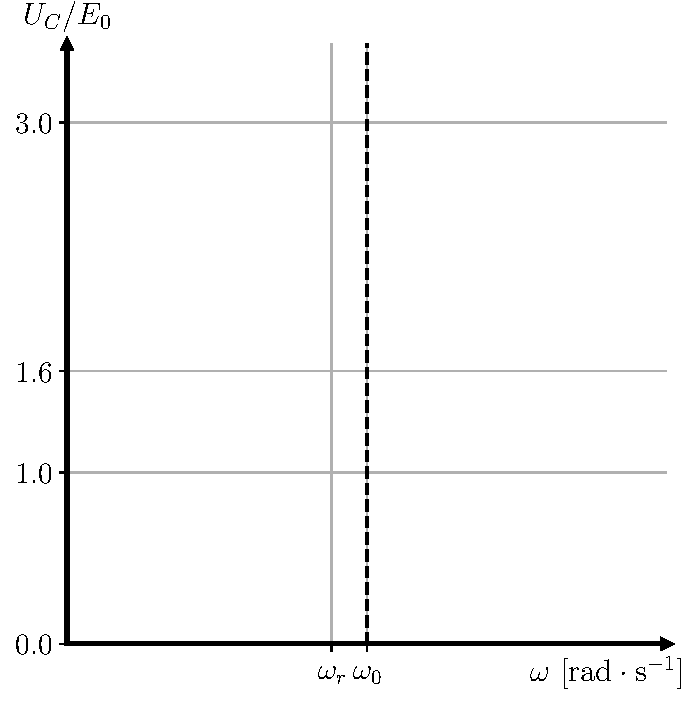
\includegraphics[width=.75\linewidth]{rlc_Uc_ampl_stud}
	}{
		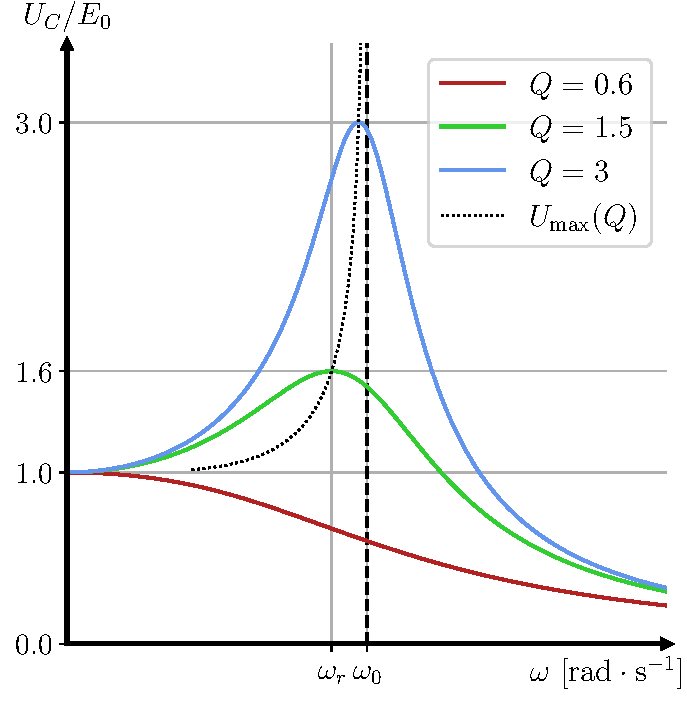
\includegraphics[width=.75\linewidth]{rlc_Uc_ampl_prof}
	}
	\\\hdashline
	\textbf{Courbes de phase} &
	\sswitch{
		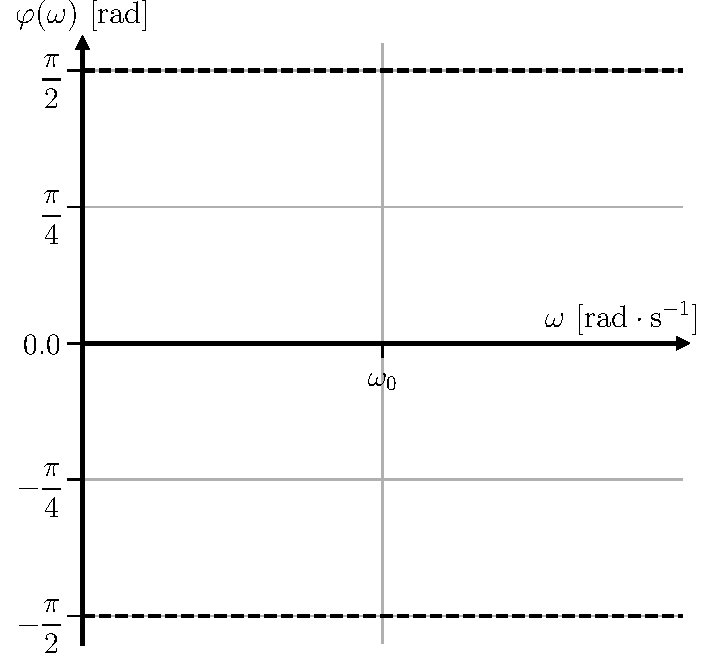
\includegraphics[width=.75\linewidth]{rlc_I_arg_stud}
	}{
		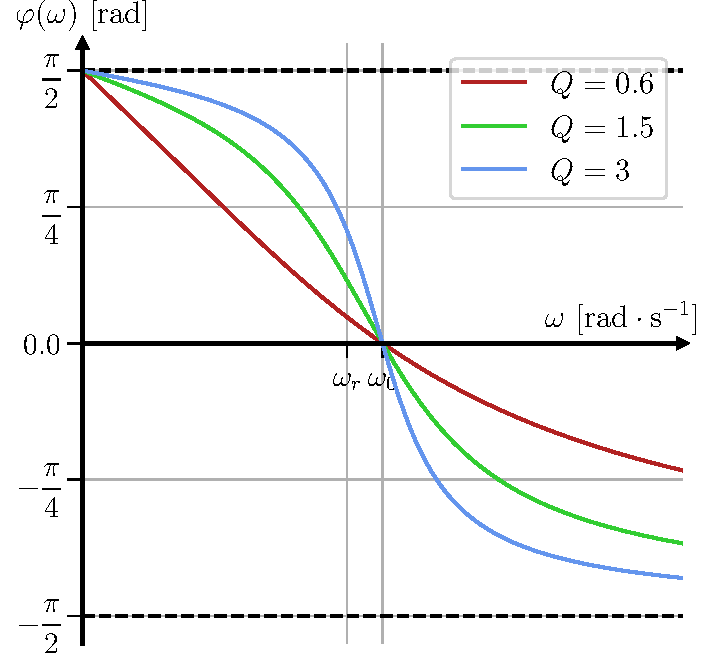
\includegraphics[width=.75\linewidth]{rlc_I_arg_prof}
	}
	&
	\sswitch{
		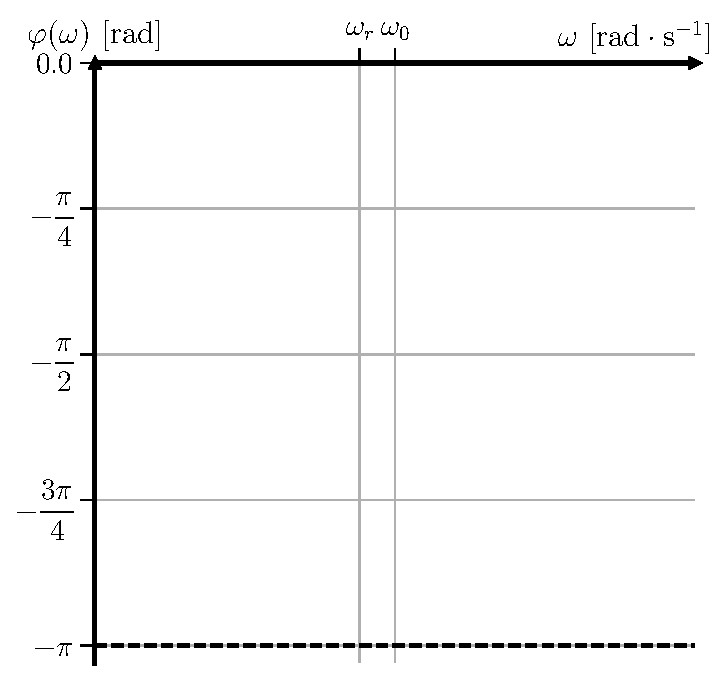
\includegraphics[width=.75\linewidth]{rlc_Uc_arg_stud}
	}{
		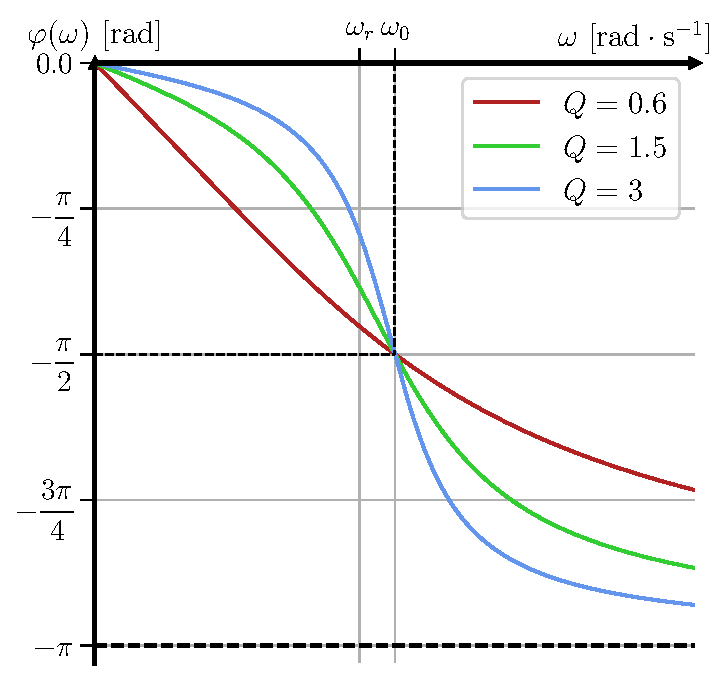
\includegraphics[width=.75\linewidth]{rlc_Uc_arg_prof}
	}
\end{tcb}
\vspace{-15pt}
\end{document}
